\documentclass[10pt,a4paper]{article}
\usepackage[utf8]{inputenc}
\usepackage[T1]{fontenc}
\usepackage{lmodern}
\usepackage{microtype}
\usepackage[a4paper,top=15mm,bottom=16mm,left=16mm,right=16mm,headheight=13pt,headsep=5mm,footskip=8mm]{geometry}
\usepackage{amsmath,amssymb,amsfonts}
\usepackage{booktabs}
\usepackage{array}
\usepackage{graphicx}
\usepackage{xcolor}
\usepackage{fancyhdr}
\usepackage{hyperref}

\definecolor{navy}{HTML}{12284C}
\definecolor{slate}{HTML}{334E68}
\definecolor{accent}{HTML}{1B5E20}
\definecolor{boxbg}{HTML}{F4F7FA}

\hypersetup{
  colorlinks=true,
  linkcolor=navy,
  urlcolor=navy,
  citecolor=navy,
  pdftitle={The Time Attraction Law: Research Monograph (Versions 1 to 21)},
  pdfauthor={David Szabolcsi}
}

\pagestyle{fancy}
\fancyhf{}
\fancyhead[L]{\footnotesize\scshape\color{slate}The Time Attraction Law --- Research Monograph (V1--V21)}
\fancyhead[R]{\footnotesize\color{slate}D\'avid Szabolcsi (ORCID: 0009-0005-6300-074X)}
\fancyfoot[L]{\footnotesize\color{slate}CC BY-NC 4.0 --- Intermediate Research Working Document (Oct 2026)}
\fancyfoot[R]{\footnotesize\bfseries\color{navy}Page \thepage\ of 15}
\renewcommand{\headrulewidth}{0.4pt}
\renewcommand{\footrulewidth}{0.4pt}

\setlength{\parindent}{0pt}
\setlength{\parskip}{2.8pt}

\newcommand{\chaphead}[2]{%
  \noindent{\color{navy}\rule{\linewidth}{1.1pt}}\par\vspace{1.5pt}%
  \noindent{\Large\bfseries\color{navy}#1}\par\vspace{1pt}%
  \noindent{\footnotesize\itshape\color{slate}#2}\par\vspace{1.5pt}%
  \noindent{\color{navy}\rule{\linewidth}{0.4pt}}\par\vspace{3pt}%
}

\begin{document}

% ==================== PAGE 1: TITLE PAGE ====================
\thispagestyle{empty}
\vspace*{1mm}
\noindent{\color{navy}\rule{\linewidth}{2pt}}\par\vspace{1.5mm}
\begin{center}
  {\footnotesize\scshape\color{slate}Intermediate Research Monograph $\cdot$ Observational, Compact-Object \& Laboratory Program}\par\vspace{1.5mm}
  {\LARGE\bfseries\color{navy}THE TIME ATTRACTION LAW}\par\vspace{2mm}
  {\large\bfseries\color{slate}Density-Modulated Time Flow, the $C$ Coupling Constant, Positive-Definite 3D Top-Hat Smoothing,}\\
  {\large\bfseries\color{slate}Galactic Rotation Curves, Multi-Source Gamma-Ray Timing, Neutron-Star Equilibrium,}\\
  {\large\bfseries\color{slate}and Laboratory Atomic-Clock \& Eight-Coil Magnetic-Field Experiments}\par\vspace{2mm}
  {\normalsize\bfseries D\'avid Szabolcsi}\par\vspace{1mm}
  {\small Independent Researcher, Unterterzen, Switzerland}\par
  {\small ORCID: \href{https://orcid.org/0009-0005-6300-074X}{\texttt{0009-0005-6300-074X}} $\cdot$ GitHub: \href{https://github.com/unbekanntedavid-glitch/Time-Attraction}{\texttt{unbekanntedavid-glitch/Time-Attraction}}}\par
  {\small October 24, 2026}
\end{center}
\vspace{1.5mm}
\noindent{\color{navy}\rule{\linewidth}{0.8pt}}\par\vspace{2mm}

{\small\noindent{\bfseries\color{navy}Overview}\par
I present the \textbf{Time Attraction Law} as an open research programme built around a specified density-smoothing prescription, developed across twenty-one iterative research stages (Versions 1 through 21). The calculations in this concise research monograph test selected equilibrium and observational couplings; they do not yet establish a covariant theory or an experimental detection of an additional clock effect. Throughout the text, I distinguish algebraic results from model assumptions and numerical checks from experimental evidence: the archived calculations document what has been tested, while the open tasks identify what is still needed to connect these results to a common dynamics. My core physical premise is that time is the primary physical medium whose local flow density is attracted and slowed by surrounding mass-energy density. Here I summarize the physical motivation (and the separate speculative bio-coherence hypothesis explored in V13--V16), the Cauchy exponential form and the \textbf{$C$ coupling constant}, the positive-definite 3D spherical top-hat law, conditional scale estimates across SPARC galaxies, the Solar System, neutron stars, and the $300\,\text{mm}$ 8-coil and granite-chamber laboratory setup, the open physical tasks (a)--(d), and the AI-assisted technical reproduction audit attached in the Appendix.

\vspace{1.5mm}
\noindent{\bfseries\color{navy}Primary Reproducible Archive Records (Zenodo DOIs \& Repository Lineage)}
\begin{center}\vspace{-2pt}
{\footnotesize
\begin{tabular}{@{}>{\bfseries}p{0.15\linewidth}p{0.27\linewidth}p{0.53\linewidth}@{}}
\toprule
Stage & Zenodo DOI / Identifier & Core Scientific Scope \& Audited Contents \\
\midrule
V1--V13 & GitHub Series Archive & Cauchy exponential ansatz, weak-field/Horndeski mappings, early time-dilation tests. \\
V14--V16 & \texttt{10.5281/zenodo.23217189} & Density-Dependent Time Coherence, $C$ coupling constant multiplier, bio-coherence $\Phi_t$ layer. \\
V17 & \texttt{10.5281/zenodo.19666220} & 155-galaxy SPARC rotation-curve processing (123 blind) \& multi-source H.E.S.S. timing audit. \\
V19 (7th Model) & \texttt{10.5281/zenodo.23497128} & Positive-definite 3D spherical top-hat law $f_L=\exp(-\gamma_L\bar{\rho}_L)$ across all 175 SPARC galaxies. \\
V20 (GH V18) & \texttt{10.5281/zenodo.23540741} & 8-coil magnetic-field energetics ($\Delta y=-1.2017\times 10^{-48}$) \& $8558\,\text{kg}$ granite clock chamber. \\
V21 (GH V19/21) & \texttt{10.5281/zenodo.23602501} & 33 neutron-star TOV sequences, Chandrasekhar radial stability, Sirius B / NICER \& open tasks. \\
\bottomrule
\end{tabular}}
\end{center}

\vspace{1mm}
\noindent{\bfseries\color{navy}Three Central Physical Questions Addressed in This Monograph}
\begin{itemize}\setlength{\itemsep}{1.5pt}\setlength{\parskip}{0pt}\setlength{\topsep}{1pt}
  \item \textbf{1. Why does clock rate shift? (The Physical ``Why''):} In Chapter 2, I address whether the Time Attraction Law represents a scalar field, an effective temporal fluid, or a refractive spacetime medium, and I explain how the algebraically locked ``how'' ($f_L = \exp(-\gamma_L \bar{\rho}_L)$) connects to the open covariant action closure (Task \texttt{50aa2db0}).
  \item \textbf{2. How does it fit across scales? (Galaxies, Solar System, and the $300\,\text{mm}$ Lab Boundary):} In Chapters 4, 5, and 10, I show how the 3D spherical top-hat kernel links galactic kiloparsec scales, unperturbed Solar System planetary ephemerides, and laboratory measurements at the $300\,\text{mm}$ coil flange boundary and $8558\,\text{kg}$ granite chamber.
  \item \textbf{3. What unique predictions distinguish it from $\Lambda$CDM?:} In Chapters 6--10, I quantify forward predictions for VHE gamma-ray arrival bounds, compact-object mass-radius and radial pulsation shifts, and polarity-even laboratory clock shifts that standard $\Lambda$CDM does not produce.
\end{itemize}

}\vfill
\noindent{\color{navy}\rule{\linewidth}{0.6pt}}\par
\noindent{\scriptsize\color{slate}\textbf{License \& Rights Notice:} This work is licensed under Creative Commons Attribution-NonCommercial 4.0 International (\textbf{CC BY-NC 4.0}). All commercial, industrial, and technological implementation rights are expressly retained by the author, D\'avid Szabolcsi.}
\newpage

% ==================== PAGE 2: TABLE OF CONTENTS & POSTURE ====================
\chaphead{Table of Contents \& Notation}{Structure of the Monograph, Fundamental Quantities, and Methodological Framework}

\noindent{\bfseries\color{navy}Contents of This Monograph}\par\vspace{1pt}
{\footnotesize
\begin{tabular}{@{}>{\bfseries\color{navy}}p{0.12\linewidth}p{0.76\linewidth}>{\raggedleft\arraybackslash\bfseries}p{0.08\linewidth}@{}}
\toprule
Section & Chapter Title & Page \\
\midrule
Title & Title Page, Overview \& Reproducible Archive Lineage & 1 \\
TOC & Table of Contents, Notation \& Methodological Principles & 2 \\
Chapter 1 & Version History from V1 to V21: The Evolution of My Research Program & 3 \\
Chapter 2 & Core Essence of the Theory: The Physical ``Why'' \& Consciousness Coherence & 4 \\
Chapter 3 & Derivation of the $C$ Coupling Constant and Cauchy Exponential Law & 5 \\
Chapter 4 & Resolution of the Negative Density Problem \& Cross-Scale Fitting & 6 \\
Chapter 5 & Galactic Rotation Curves: Processing 155 SPARC Galaxies \& 3D Top-Hat Grids & 7 \\
Chapter 6 & Very-High-Energy Gamma-Ray Timing: Multi-Source H.E.S.S. Data Analysis & 8 \\
Chapter 7 & Neutron-Star Modeling in V21: TOV Sequences \& NICER Mass--Radius Bounds & 9 \\
Chapter 8 & Perturbation Calculations: Anisotropic Stress \& Chandrasekhar Radial Stability & 10 \\
Chapter 9 & Conditional Clock \& Redshift Hypotheses: Sirius B and NICER Likelihoods & 11 \\
Chapter 10 & Planned Laboratory Measurements: Eight-Coil Field \& Granite Clock Chamber & 12 \\
Chapter 11 & Open Theoretical and Experimental Questions: Laboratory \& Theoretical Tasks (a)--(d) & 13 \\
Chapter 12 & Closing Chapter: The Immediate Next Physical Step of the Research Program & 13 \\
Appendix & AI-Assisted Technical Reproduction Audit (English Translation, \texttt{revision3\_review\_EN.md}) & 14--15 \\
\bottomrule
\end{tabular}}

\vspace{1.5mm}
\noindent{\bfseries\color{navy}Core Concepts and Mathematical Symbols}\par
To maintain clarity across all historical stages, this monograph uses the following notation throughout:
\begin{center}\vspace{-2pt}
{\footnotesize
\begin{tabular}{@{}>{\bfseries}p{0.28\linewidth}p{0.24\linewidth}p{0.43\linewidth}@{}}
\toprule
Concept & Symbol / Definition & Physical Role in the Time Attraction Law \\
\midrule
Time Attraction Law & $f_L(\mathbf{x}) = \exp(-\gamma_L \bar{\rho}_L(\mathbf{x}))$ & Universal law relating local time-flow density to smoothed mass-energy density. \\
$C$ coupling constant & $C \equiv \frac{4\pi G}{c^2} = 9.331988\times 10^{-27}\,\text{m/kg}$ & Defined geometric-gravitational coupling constant ($G/c^2 = 7.426160\times 10^{-28}\,\text{m/kg}$; distinct from historical amplifier $C_{\text{amp}}(\rho)$). \\
Scale coupling ($\alpha=1$) & $\gamma_L = \alpha\frac{G L^2}{c^2} = \frac{C L^2}{4\pi}\;(\alpha=1)$ & Scale-dependent damping coefficient ($\text{m}^3\,\text{kg}^{-1}$) for smoothing radius $L$ (distinct from likelihood $\mathcal{L}_{\text{like}}$). \\
3D top-hat density & $\bar{\rho}_L(\mathbf{x}) = \frac{3}{4\pi L^3}\int_{|\mathbf{y}-\mathbf{x}|\le L}\rho(\mathbf{y})\,d^3y$ & Non-negative spherical average of mass density $\rho$ (or energy density $\varepsilon/c^2$), resolving $\rho<0$. \\
Consciousness coherence & $\Phi_t,\,\Phi_B,\,\kappa$ & Early-stage theoretical bio-coherence resonance potential, magnetic flux, curvature. \\
\bottomrule
\end{tabular}}
\end{center}

\vspace{2mm}
\noindent{\bfseries\color{navy}Methodological Principles: Reproducibility and Open Questions}\par
In presenting this gravitational and temporal framework, I maintain a strict separation between what I have already locked down in hash-verified, reproducible code and what remains an open theoretical or experimental task:
\begin{enumerate}\setlength{\itemsep}{2pt}\setlength{\parskip}{0pt}\setlength{\topsep}{2pt}
  \item \textbf{The Audited ``How'' Is Reproducibly Locked:} Across my Zenodo records and GitHub repository, I have provided deterministic scripts, SHA-256 manifests, and independent quadrature checks that define \emph{how} the Time Attraction Law maps mass-energy density $\rho(\mathbf{x})$ into the bounded attenuation factor $0 < f_L(\mathbf{x}) \le 1$.
  \item \textbf{Every Version Is an Intermediate Step:} No release in my V1--V21 sequence is treated as closed. Each version tests a specific mathematical hypothesis against observational or laboratory constraints, documents its limitations openly, and refines the formulation accordingly.
  \item \textbf{AI-Assisted Technical Reproduction Audits:} Technical reproduction and manuscript audits conducted with Academia Co-scientist (not institutional journal peer review) served as diagnostic instruments. When those checks flagged the 1D midplane proxy vs.\ 3D top-hat distinction in V19, the magnetic cross-term $2\mathbf{B}_{\text{bg}}\cdot\mathbf{B}_{\text{coil}}$ in V20, or the approximate pulsation operators and open covariant action closure in V21, I updated my code and documentation accordingly. The English translation of the Round-3 technical audit is reproduced on Pages 14 and 15.
\end{enumerate}
\newpage

% ==================== PAGE 3: CHAPTER 1 (VERSION HISTORY V1-V21) ====================
\chaphead{Chapter 1: Version History from V1 to V21}{Tracing the Iterative Path of the Time Attraction Law Across Twenty-One Research Stages}

To allow the reader to follow the exact trajectory of my research, I summarize here how the \textbf{Time Attraction Law} evolved from its initial mathematical ansatz in Version 1 to the multi-messenger, compact-object, and laboratory packages in Version 21. Every stage served as a stepping stone that exposed what worked and what needed correction.

\begin{center}\vspace{-2pt}
{\footnotesize
\begin{tabular}{@{}>{\bfseries\color{navy}}p{0.14\linewidth}p{0.25\linewidth}p{0.56\linewidth}@{}}
\toprule
Version Stage & Primary Focus & Milestones Achieved, Lessons Learned \& Self-Corrections \\
\midrule
V1 -- V4 & Cauchy Multiplicative Ansatz & I formulated the postulate that independent local mass densities compound multiplicatively on time flow, $f(\rho_1+\rho_2)=f(\rho_1)f(\rho_2)$, yielding $f(\rho)=\exp(-\gamma\rho)$. \\
V5 -- V7 & Weak-Field \& Chameleon Explorations & I explored scalar-tensor and chameleon-like screening analogies to connect local density gradients with effective gravitational accelerations in low-density environments. \\
V8 -- V12 & Horndeski \& Time-Dilation Mappings & I investigated effective metric lapse modifications and Horndeski-inspired scalar couplings, testing whether optical clock comparisons could bound the coupling scale. \\
V13 -- V16 & Density-Dependent Time Coherence \& Bio-Coherence ($\Phi_t$) & (\texttt{10.5281/zenodo.23217189}) I introduced the \textbf{$C$ coupling constant} ($C=4\pi G/c^2$), the force multiplier $C(\rho)=1+C_0 e^{-\rho/\rho_c}$ ($C_0=5$), and the consciousness-coherence bridge ($\Phi_t$, $\Phi_B$, $\kappa$, EEG/HRV bio-coherence). Subsequent self-audits showed that linear differential forms could trigger $\rho<0$ sign inversions and that $C_0=5$ over-predicted flat rotation curves. \\
V17 & SPARC 155-Galaxy \& H.E.S.S. Multi-Source Audit & (\texttt{10.5281/zenodo.19666220}) I audited 175 SPARC galaxies (155 quality-filtered rotation curves; 123 blind test galaxies with 2596 points) and multi-source H.E.S.S. VHE gamma-ray flares (PKS 2155-304, Mrk 501, Vela, Crab, GRB 190114C), replacing single-flare claims with rigorous multi-source controls. \\
V18 (Internal) & Smoothing-Kernel Reformulation & I tested integral smoothing kernels to eliminate numerical derivative noise and prevent unphysical negative effective densities near sharp density boundaries. \\
V19 (7th Model) & Positive-Definite 3D Spherical Top-Hat Law & (\texttt{10.5281/zenodo.23497128}) I resolved the negative-density problem by defining $\bar{\rho}_L(\mathbf{x})$ as a 3D spherical top-hat integral over radius $L$, guaranteeing $\bar{\rho}_L\ge 0$ and $0<f_L\le 1$, and evaluated it across all 175 SPARC galaxies. \\
V20 (GH V18) & 8-Coil Magnetic Field \& Granite Clock Chamber & (\texttt{10.5281/zenodo.23540741}) I designed the terrestrial laboratory program: an $8558\,\text{kg}$ movable granite chamber around an atomic clock and an 8-coil magnetic-field energetics test ($\varnothing 300\,\text{mm}$ flange boundary, $\Delta y = -1.2017108\times 10^{-48}$ at $L=0.631\,\text{m}$), checked across three AI-assisted technical reproduction audit rounds. \\
V21 (GH V19/21) & Neutron-Star TOV, Perturbations \& Open Tasks & (\texttt{10.5281/zenodo.23602501}) I extended the 3D top-hat law to 33 neutron-star TOV sequences (SLy, APR4, H4), X-sector anisotropic stress reconstruction, Chandrasekhar radial stability ($\omega_0^2$), Sirius B / NICER conditional tests, and four explicit open physical tasks (a)--(d). \\
\bottomrule
\end{tabular}}
\end{center}

\noindent{\bfseries\color{navy}Three Turning Points in My Iterative Research Journey}\par
Looking back across V1--V21, three methodological turning points define the maturity of the work:
\begin{enumerate}\setlength{\itemsep}{1.5pt}\setlength{\parskip}{0pt}\setlength{\topsep}{1pt}
  \item \textbf{From Differential Proxies to Positive-Definite Integral Smoothing (V13 $\to$ V19):} In early versions, evaluating Laplacians or local midplane proxies produced sign inversions where effective density dropped below zero. By introducing the 3D spherical top-hat average $\bar{\rho}_L$ in V19, I mathematically guaranteed $0 < f_L(\mathbf{x}) \le 1$ at every point in space.
  \item \textbf{From Single-Dataset Fits to Blind Multi-Object Controls (V16 $\to$ V17/V19):} Rather than tuning parameters to individual galaxies or a single blazar flare, I locked the stellar mass-to-light ratios ($\Upsilon_{\text{disk}}=0.5$, $\Upsilon_{\text{bulge}}=0.7\,M_\odot/L_\odot$) across the SPARC sample and cross-checked PKS 2155-304 against four additional H.E.S.S. gamma-ray sources.
  \item \textbf{From Algebraic Prescriptions to Explicit Open Boundary Conditions (V20 $\to$ V21):} In V20 and V21, I paired every numerical calculation with SHA-256 verification manifests and explicitly separated locked algebraic profiles from the open covariant action derivation (Task \texttt{50aa2db0}).
\end{enumerate}
\newpage

% ==================== PAGE 4: CHAPTER 2 (CORE ESSENCE, PHYSICAL WHY & CONSCIOUSNESS COHERENCE) ====================
\chaphead{Chapter 2: Core Essence of the Theory --- The Physical ``Why'' \& Consciousness Coherence}{Why Time Flow Is Modulated by Mass-Energy Density, the Medium Interpretation, and the Bio-Coherence Layer}

A physical theory cannot stop at describing \emph{how} a curve bends; it must address \emph{why} the effect occurs. In the \textbf{Time Attraction Law}, I start from a foundational ontological shift: \textbf{time is not a passive, uniform mathematical coordinate, but the primary physical carrier whose local flow density is attracted and compressed by mass-energy density.}

\noindent{\bfseries\color{navy}1. The Physical ``Why'': Field, Temporal Fluid, or Refractive Spacetime Medium?}\par
In standard general relativity, mass-energy curves spacetime geometry via $G_{\mu\nu} = \frac{8\pi G}{c^4}T_{\mu\nu}$, and gravitational time dilation emerges purely from the metric component $g_{00}$. In my framework, I ask what physical mechanism underlies the local slowing of clocks when mass-energy accumulates within an interaction neighborhood of radius $L$. I interpret time flow as possessing an effective local carrier density (analogous to an optical medium with refractive index $n_t(\mathbf{x}) = f_L(\mathbf{x})^{-1} = \exp(+\gamma_L \bar{\rho}_L(\mathbf{x}))$ or a compressible temporal fluid). Wherever mass-energy density $\rho(\mathbf{x}) = T_{00}/c^2$ concentrates, it attracts and condenses the temporal medium inside the causal averaging sphere of radius $L$. Consequently, the local rate of proper time progression relative to a vacuum reference clock is attenuated by:
\begin{equation}
  f_L(\mathbf{x}) \;=\; \exp\!\bigl(-\gamma_L\,\bar{\rho}_L(\mathbf{x})\bigr), \qquad \gamma_L \;=\; \frac{G L^2}{c^2} \;=\; \frac{C\,L^2}{4\pi},
\end{equation}
where $C = 4\pi G/c^2$ is the \textbf{$C$ coupling constant}. In this picture, gravity is not merely geometric curvature in a vacuum; it is the macroscopic manifestation of gradients in the density of time flow.

\noindent{\bfseries\color{navy}2. Separating the Audited ``How'' from the Dynamical ``Why'' (Task \texttt{50aa2db0})}\par
Scientific integrity requires distinguishing between what is already algebraically verified and what requires a deeper field-theoretical derivation. In V19--V21, I locked the functional \textbf{``how''}---the exact non-local mapping from $\rho(\mathbf{x})$ to $\bar{\rho}_L(\mathbf{x})$ and $f_L(\mathbf{x})$, verified to $10^{-15}$ numerical precision. In the audited neutron-star recipes, the hydrostatic balance $P' = -(\varepsilon+P)\nu'$ guarantees that the matter stress-energy tensor is conserved on its own ($\nabla_\mu T^{\mu\nu}_{\text{matter}} = 0$). However, modifying the metric functions ($\nu'$ or $m'$) by $f_L(r)$ without a full field action leaves the right-hand side of the Einstein equations unclosed unless supplemented by an effective stress-energy tensor $T^{\mu\nu}_X$ satisfying $\nabla_\mu G^{\mu\nu} = 8\pi\nabla_\mu(T^{\mu\nu}_{\text{matter}} + T^{\mu\nu}_X) = 0$. Therefore, the dynamical \textbf{``why''} is formulated as Task \texttt{50aa2db0}: deriving the background equations, $X$-sector, and matter couplings from a single covariant action principle.

\noindent{\bfseries\color{navy}3. Speculative Hypothesis Layer: The Consciousness-Coherence Bridge ($\Phi_t$, $\Phi_B$, $\kappa$)}\par
In Versions 13 through 16 (and preserved in the theoretical lineage of V17), I also explored a broader, speculative unification question: if the local density of time flow is a physical medium modulated by mass and energy, can coherent electromagnetic and biological information structures couple to that same temporal carrier? In that extended theoretical layer, I introduced the \textbf{consciousness-coherence resonance potential} $\Phi_t$ alongside magnetic flux $\Phi_B$ and spatial curvature $\kappa$, writing a generalized effective source density and total stress-energy tensor:
\begin{equation}
  \rho_{\text{eff}} \;=\; \rho \;+\; \Xi\,\varepsilon_0\,\Phi_t \;+\; \beta\,\Phi_B \;+\; \gamma\,\kappa, \qquad
  T_{\mu\nu}^{\text{total}} \;=\; T_{\mu\nu}^{\text{matter}} \;+\; T_{\mu\nu}^{\text{flux}} \;+\; T_{\mu\nu}^{\text{thought}},
\end{equation}
where $\Xi$ denotes the temporal-coherence coupling coefficient and $\varepsilon_0$ is the vacuum permittivity. Within this hypothesis, biological neural and cardiac oscillators (quantified via phase-locked EEG gamma/theta synchrony and heart-rate variability, HRV, bio-coherence indices) act as ultra-sensitive phase detectors of local temporal coherence. Specifically, the theoretical model proposes that fluctuations in local mass-energy density $\rho$, geomagnetic/coil flux $\Phi_B$, and shielding geometry could induce measurable shifts in EEG/HRV phase coherence.

\noindent{\bfseries\color{navy}4. Strict Methodological Boundary Between Audited Physics and Perspective Extensions}\par
In my research program, I maintain a clear boundary between the two layers:
\begin{itemize}\setlength{\itemsep}{1.5pt}\setlength{\parskip}{0pt}\setlength{\topsep}{1pt}
  \item \textbf{Audited Physical Core (V19--V21):} All quantitative claims in my SPARC galactic rotation analysis, H.E.S.S. timing bounds, neutron-star TOV and pulsation sequences, and the V20 granite-chamber and 8-coil quartz oscillator laboratory protocol rely \emph{exclusively} on standard baryonic and electromagnetic mass-energy density $\rho = T_{00}/c^2$, with $\Phi_t \equiv 0$.
  \item \textbf{Perspective Bio-Coherence Layer (V13--V16):} The consciousness-coherence terms ($\Phi_t$, $T_{\mu\nu}^{\text{thought}}$, EEG/HRV bio-coherence) remain an open, un-audited theoretical perspective recorded as part of the historical intellectual trajectory of the Time Attraction Law.
\end{itemize}
\newpage

% ==================== PAGE 5: CHAPTER 3 (DERIVATION OF THE C COUPLING CONSTANT) ====================
\chaphead{Chapter 3: Exponential Form, Definition of $C$, and Normalization}{Cauchy Functional-Equation Derivation of the Exponential Law, Definition of $C$, and the $\alpha=1$ Postulate}

Here I separate three distinct mathematical elements: (1) deriving the exponential functional form from multiplicative postulates, (2) defining the constant $C \equiv 4\pi G/c^2$, and (3) adopting the dimensional normalization postulate $\alpha = 1$ in $\gamma_L = \alpha (G/c^2)L^2$, followed by my self-audit of the historical V14--V16 amplifier $C_{\text{amp}}(\rho)$.

\noindent{\bfseries\color{navy}1. Derivation of the Exponential Law from Cauchy's Functional Equation}\par
Consider a reference clock in vacuum ($\rho = 0$) ticking at proper rate $d\tau_0$, and an identical clock placed inside a region whose smoothed mass-energy density within radius $L$ is $\bar{\rho}_L \ge 0$. Let $f(\bar{\rho}_L) = d\tau / d\tau_0$ denote the dimensionless time-flow attenuation factor. I impose three physical axioms:
\begin{enumerate}\setlength{\itemsep}{1pt}\setlength{\parskip}{0pt}\setlength{\topsep}{1pt}
  \item \textbf{Vacuum Normalization:} In the absence of mass-energy ($\bar{\rho}_L = 0$), time flows at the unattenuated reference rate, so $f(0) = 1$.
  \item \textbf{Multiplicative Superposition:} If two independent, non-overlapping mass distributions contribute smoothed densities $\rho_1$ and $\rho_2$ within the interaction sphere, the sequential attenuation of the temporal carrier is multiplicative:
  \begin{equation}
    f(\rho_1 + \rho_2) \;=\; f(\rho_1)\,f(\rho_2) \qquad \forall\,\rho_1,\rho_2 \ge 0.
  \end{equation}
  \item \textbf{Monotonic Attraction (Slowing of Time Flow):} Increasing mass-energy density attracts and condenses the temporal medium, slowing the local clock rate: $0 < f(\rho) \le 1$ and $df/d\rho < 0$.
\end{enumerate}
By Cauchy's classical theorem on continuous solutions of $f(x+y)=f(x)f(y)$ on $[0,\infty)$, the unique continuous solution satisfying $f(0)=1$ and $df/d\rho < 0$ is the pure real exponential:
\begin{equation}
  f_L(\bar{\rho}_L) \;=\; \exp\!\bigl(-\gamma_L\,\bar{\rho}_L\bigr), \qquad \gamma_L > 0, \qquad [\gamma_L] \;=\; \text{m}^3\,\text{kg}^{-1}.
\end{equation}

\noindent{\bfseries\color{navy}2. Definition of the $C$ Coupling Constant and the $\alpha = 1$ Normalization Assumption}\par
Cauchy's theorem fixes the exponential shape (4) with a free positive constant $\gamma_L > 0$, but does not by itself fix its normalization. Using CODATA values $G = 6.67430\times 10^{-11}\,\text{m}^3\,\text{kg}^{-1}\,\text{s}^{-2}$ and $c = 299\,792\,458\,\text{m}\,\text{s}^{-1}$, the gravitational mass-to-length ratio is $G/c^2$, and I define the \textbf{$C$ coupling constant} as its $4\pi$ spherical counterpart:
\begin{equation}
  C \;\equiv\; \frac{4\pi G}{c^2} \;=\; 9.3319882\times 10^{-27}\;\text{m}\,\text{kg}^{-1}, \qquad
  \frac{G}{c^2} \;=\; \frac{C}{4\pi} \;=\; 7.4261603\times 10^{-28}\;\text{m}\,\text{kg}^{-1}.
\end{equation}
Dimensional analysis allows $\gamma_L = \alpha\,(G/c^2)\,L^2$ with any dimensionless constant $\alpha > 0$. Setting $\alpha = 1$ is an explicit model normalization assumption (not a purely algebraic consequence of Cauchy's equation), yielding:
\begin{equation}
  \gamma_L \;=\; \frac{G\,L^2}{c^2} \;=\; \frac{C\,L^2}{4\pi} \;=\; 7.4261603\times 10^{-28}\,L^2\;\text{m}^3\,\text{kg}^{-1}\quad(\text{for }\alpha=1).
\end{equation}
Here $f_L$ denotes the local TAL attenuation factor; in curved spacetime (Chapter 9), standard GR redshift $e^{\nu/2}$ is either modified solely via the hydrostatic metric (H0) or multiplied by $f_L(R_*)$ as an explicit conditional clock hypothesis (H1).

\noindent{\bfseries\color{navy}3. Empirical Re-Evaluation of the V14--V16 Historical Amplifier $C_{\text{amp}}(\rho) = 1 + C_0\exp(-\rho/\rho_c)$}\par
In Versions 14--16 (DOI \texttt{10.5281/zenodo.23217189}), before I introduced the 3D spherical top-hat integral, I explored a phenomenological weak-field force multiplier of the form:
\begin{equation}
  v_{\text{rot}}^2(r) \;=\; v_{\text{baryon}}^2(r)\cdot C(\rho(r)), \qquad C(\rho) \;=\; 1 \;+\; C_0\,\exp\!\left(-\frac{\rho}{\rho_c}\right),
\end{equation}
with a fixed amplitude $C_0 = 5$ (so $C(\rho)\to 6$ in ultra-low-density outskirts $\rho \ll \rho_c$) and a critical threshold density $\rho_c$. During the V17 audit (DOI \texttt{10.5281/zenodo.19666220}), I subjected this formula to a blind test across 123 SPARC galaxies and discovered two critical limitations:
\begin{itemize}\setlength{\itemsep}{1.5pt}\setlength{\parskip}{0pt}\setlength{\topsep}{1pt}
  \item \textbf{Empirical Over-Prediction:} Fixing $C_0=5$ boosts asymptotic velocities by $\sqrt{6}\approx 2.45$, which systematically overshoots intermediate-surface-brightness galaxies and degrades the median reduced $\chi^2_\nu$ from $2.898$ (baryonic baseline) to $9.39$ across the 123-galaxy blind sample.
  \item \textbf{Local Pointwise Instability:} Evaluating $\rho(r)$ pointwise or via thin-disk derivatives introduces sensitivity to local gas clumps and sign inversions. This realization directly motivated my transition to the parameter-free 3D spherical top-hat integral in Version 19.
\end{itemize}
\newpage

% ==================== PAGE 6: CHAPTER 4 (NEGATIVE DENSITY RESOLUTION & CROSS-SCALE FITTING) ====================
\chaphead{Chapter 4: Resolution of the Negative Density Problem \& Cross-Scale Fitting}{My 7th Model (V19 3D Spherical Top-Hat Law) and How the Theory Connects Galaxies, the Solar System, and the Lab}

\noindent{\bfseries\color{navy}1. Why Early Formulations Suffered from Negative Densities ($\rho < 0$ or $f < 0$)}\par
In early iterations of my research (and in standard first-order weak-field expansions where $\exp(-\gamma\rho) \approx 1 - \gamma\rho$ or where effective densities are reconstructed from the Laplacian $\nabla^2\Phi_{\text{eff}}$ near sharp disk edges), two mathematical pathologies arose:
\begin{enumerate}\setlength{\itemsep}{1pt}\setlength{\parskip}{0pt}\setlength{\topsep}{1pt}
  \item \textbf{Linearized Sign Inversion ($f_{\text{lin}} < 0$):} In high-density regimes (such as neutron-star cores where $\rho \sim 10^{18}\,\text{kg/m}^3$) or at large smoothing scales $L$, the linear Taylor approximation $1 - \gamma_L\rho$ crosses zero and becomes negative whenever $\gamma_L\rho > 1$, reversing the sign of time flow.
  \item \textbf{Differential Deconvolution Oscillations ($\rho_{\text{eff}} < 0$):} Computing effective densities from second derivatives of noisy rotation curves or oscillatory Bessel kernels produces unphysical regions of negative mass density ($\rho_{\text{eff}} < 0$) outside truncated stellar disks or coil flanges.
\end{enumerate}

\noindent{\bfseries\color{navy}2. My Solution in Version 19 (7th Model): The 3D Spherical Top-Hat Integral}\par
In Version 19 (DOI \texttt{10.5281/zenodo.23497128}), I resolved both pathologies permanently by formulating the \textbf{7th Model} of the Time Attraction Law. Instead of evaluating pointwise derivatives or linear approximations, I define the source of temporal attenuation at any position $\mathbf{x} \in \mathbb{R}^3$ as the unweighted three-dimensional spherical top-hat average of the physical mass-energy density $\rho(\mathbf{y}) = T_{00}(\mathbf{y})/c^2 \ge 0$ inside a ball $B(\mathbf{x},L)$ of radius $L > 0$:
\begin{equation}
  \bar{\rho}_L(\mathbf{x}) \;\equiv\; \frac{3}{4\pi L^3}\int_{|\mathbf{y}-\mathbf{x}|\le L} \rho(\mathbf{y})\,d^3y \;=\; \frac{M_{\text{enc}}(\mathbf{x};L)}{\frac{4}{3}\pi L^3}, \qquad
  f_L(\mathbf{x}) \;=\; \exp\!\bigl(-\gamma_L\,\bar{\rho}_L(\mathbf{x})\bigr).
\end{equation}
Because physical mass-energy density satisfies $\rho(\mathbf{y}) \ge 0$ everywhere and the characteristic indicator function $\Theta(L - |\mathbf{y}-\mathbf{x}|)$ is strictly non-negative, the integral $\bar{\rho}_L(\mathbf{x})$ is \textbf{positive semi-definite ($\bar{\rho}_L(\mathbf{x}) \ge 0$)} for every geometry, whether a spiral galaxy, a neutron star, or an 8-coil laboratory array. Consequently, the exponential attenuation factor obeys the exact analytical bounds:
\begin{equation}
  0 \;<\; f_L(\mathbf{x}) \;\le\; 1 \qquad \forall\,\mathbf{x}\in\mathbb{R}^3,\;\;\forall\,L > 0.
\end{equation}
No negative density, sign inversion, or metric horizon flip from $f_L$ can ever occur.

\noindent{\bfseries\color{navy}3. How Does the Time Attraction Law Fit Across Scales? (Galaxies $\to$ Solar System $\to$ $300\,\text{mm}$ Lab)}\par
A crucial question for any gravitational framework is \emph{how it fits across vastly different length scales}: if it operates in galaxies, what happens in the Solar System, and why does the laboratory test at the $300\,\text{mm}$ coil flange boundary and $8558\,\text{kg}$ granite chamber matter? The 3D top-hat scaling law $\gamma_L \bar{\rho}_L = \frac{3 G M_{\text{enc}}(\mathbf{x};L)}{4\pi c^2 L}$ provides a unified quantitative answer across four regimes:
\begin{center}\vspace{-2pt}
{\footnotesize
\begin{tabular}{@{}>{\bfseries}p{0.20\linewidth}p{0.20\linewidth}p{0.23\linewidth}p{0.31\linewidth}@{}}
\toprule
Physical Regime & Characteristic Scale & Enclosed Mass / Density & Magnitude of $|1 - f_L|$ \& Physical Behavior \\
\midrule
Galactic Disks (SPARC 175) & $R \sim 1\text{--}50\,\text{kpc}$, $L \sim 2.37\,\text{Mpc}$ & $M_{\text{bary}} \sim 10^8\text{--}10^{11}\,M_\odot$ & Galaxy-only $\max|1-f_L| = 2.30\times 10^{-7}$; requires cosmic background or $L\sim 22.9\,\text{Gpc}$ for unit exponent. \\
Solar System Scale Estimate & $r \sim 1\text{--}30\,\text{AU}$, $L \gg 1\,\text{AU}$ & $M_\odot = 1.989\times 10^{30}\,\text{kg}$ diluted in $L^3$ sphere & Conditional scale estimate: for $L \gtrsim 1\,\text{pc}$, $\gamma_L\bar{\rho}_L^\odot \lesssim 10^{-14}$ (full orbit/light test requires Tasks a, d). \\
Compact Stars (WD / NS V21) & $R \sim 10\,\text{km}\text{--}5500\,\text{km}$, $L \sim 1\,\text{m}\text{--}100\,\text{km}$ & $\rho \sim 10^9\text{--}10^{18}\,\text{kg/m}^3$ & Strong-field regime: $1-f_L \sim 10^{-4}\text{--}0.85$; shifts NS $M$--$R$ curves and Sirius B conditional redshift. \\
Lab Chambers \& Coils (V20) & $L \sim 0.1\text{--}3\,\text{m}$, $\varnothing 300\,\text{mm}$ flange & Granite $8558\,\text{kg}$ ($\rho=2750$); 8 coils ($u_B/c^2$) & At $L=0.631\,\text{m}$, sphere encloses the $300\,\text{mm}$ flanges: $|\Delta y|_{\text{coil}}=1.20\times 10^{-48}$, $|\Delta y|_{\text{granite}}\sim 10^{-24}$. \\
\bottomrule
\end{tabular}}
\end{center}
This table provides a conditional order-of-magnitude scale comparison: for $L \gg 1\,\text{AU}$, diluting $M_\odot$ over $\frac{4}{3}\pi L^3$ makes the dimensionless exponent $\gamma_L\bar{\rho}_L^\odot$ small, though a rigorous confrontation with Cassini and planetary ephemeris bounds requires solving the coupled dynamical equations of motion and light propagation (Open Tasks (a) and (d)). In the meter-scale laboratory window ($L \sim 0.63\,\text{m}$), the averaging sphere matches the geometry of the granite chamber ($R_{\text{out}}=0.85\,\text{m}$) and the $300\,\text{mm}$ flange boundary ($291.7\,\text{mm}$ winding diameter) of the 8-coil array.
\newpage

% ==================== PAGE 7: CHAPTER 5 (SPARC 155 GALAXIES & 3D TOP-HAT GRIDS) ====================
\chaphead{Chapter 5: Galactic Rotation Curves --- Processing 155 SPARC Galaxies}{From the V17 Quality-Filtered \& Blind SPARC Audit to the V19/V20 Exact 3D Spherical Top-Hat Evaluation}

To test the \textbf{Time Attraction Law} against galactic dynamics without dark-matter halo tuning, I processed the Spitzer Photometry and Accurate Rotation Curves (SPARC) database across two major stages: the V17 statistical pipeline (DOI \texttt{10.5281/zenodo.19666220}) and the V19/V20 exact 3D spherical top-hat evaluation (DOI \texttt{10.5281/zenodo.23497128}).

\noindent{\bfseries\color{navy}1. The V17 SPARC Pipeline: 175 Total, 155 Processed, and 123 Blind-Test Galaxies}\par
The master SPARC catalog contains \textbf{175 late-type and dwarf galaxies} with surface photometry at $3.6\,\mu\text{m}$ and resolved $\text{H\,\textsc{i}}/\text{H}\alpha$ rotation curves. In my V17 processing pipeline, removing 20 systems with severe kinematic asymmetries or inclination flags ($i < 30^\circ$ or $Q=3$) yielded the \textbf{155-galaxy processed rotation-curve sample}. Enforcing strict data-hygiene cuts (requiring at least 5 radial points and full baryonic decomposition components $V_{\text{gas}}, V_{\text{disk}}, V_{\text{bulge}}$) defined the \textbf{123-galaxy blind validation sample} comprising \textbf{2,596 radial velocity measurements}. Throughout all fits, I locked the stellar mass-to-light ratios to standard population-synthesis values ($\Upsilon_{\text{disk}} = 0.5\,M_\odot/L_\odot$, $\Upsilon_{\text{bulge}} = 0.7\,M_\odot/L_\odot$) so that no galaxy-by-galaxy halo parameters were adjusted.

\noindent{\bfseries\color{navy}2. Exact 3D Spherical Top-Hat Evaluation Across All 175 SPARC Galaxies (V19)}\par
In Version 19, I replaced the thin-disk midplane proxy $\rho_{\text{mid}}(r) = \Sigma_{\text{bary}}(r)/(2h_z)$ with the exact 3D axisymmetric mass distribution $\rho_{\text{bary}}(R,z) = \frac{\Sigma_{\text{bary}}(R)}{2h_z}\exp(-|z|/h_z)$ (with scale height $h_z = 0.196\,R_d^{0.633}$) and integrated $\bar{\rho}_L(r)$ inside a 3D sphere of radius $L$ centered at every midplane radial point $(r,0,0)$. Independent referee verification confirmed three decisive numerical facts:
\begin{enumerate}\setlength{\itemsep}{1pt}\setlength{\parskip}{0pt}\setlength{\topsep}{1pt}
  \item \textbf{Galaxy-Only 3D Top-Hat Signal (\texttt{sparc\_tophat.zip}):} Because a 3D sphere of radius $L \gg h_z$ extends far into the vacuum above and below the thin galactic disk, the enclosed galactic mass is diluted by $L^3$. Across all 175 SPARC galaxies, the maximum galaxy-attributable deviation is $\max |1 - f_L| = 2.280\times 10^{-7}$ on the 81-point logarithmic $L$-grid and \textbf{$2.303\times 10^{-7}$} under continuous optimization, attained in \textbf{UGC03546} at radius $R = 0.63\,\text{kpc}$ and smoothing scale $L \approx 0.825\,\text{kpc}$ (whereas in the earlier V19 fit, UGC02487 peaked near $L \approx 23.09\,\text{kpc}$).
  \item \textbf{1D Midplane Proxy vs.\ True 3D Top-Hat at $L = 2.3714\,\text{Mpc}$ (\texttt{fitted\_L\_scores.csv}):} In the audited explicit-error pipeline at $L = 2.3714\,\text{Mpc}$, the pure baryonic baseline ($v_{\text{bar}}$) and the isolated-galaxy 3D spherical top-hat integral yield identical reduced-$\chi^2_\nu$ medians of \textbf{$2.8980$} across all $N=175$ galaxies and \textbf{$3.1433$} across the Blind-123 subsample, whereas the historical 1D midplane proxy yielded $2.6716$ ($N=175$) and $2.7082$ (Blind-123).
  \item \textbf{Homogeneous Matter Background Scale ($L_{\text{eff}} \approx 22.94\,\text{Gpc}$):} In the homogeneous cosmic matter background $\bar{\rho}_0 \approx 2.68\times 10^{-27}\,\text{kg/m}^3$ ($\Omega_m \approx 0.315, H_0 = 67.4\,\text{km/s/Mpc}$), the condition $\gamma_L\bar{\rho}_0 = 1$ corresponds to the cosmological length scale $L_{\text{eff}} = (G\bar{\rho}_0/c^2)^{-1/2} \approx 22.94\,\text{Gpc}$ ($7.08\times 10^{26}\,\text{m}$).
\end{enumerate}

\begin{center}\vspace{-4pt}
  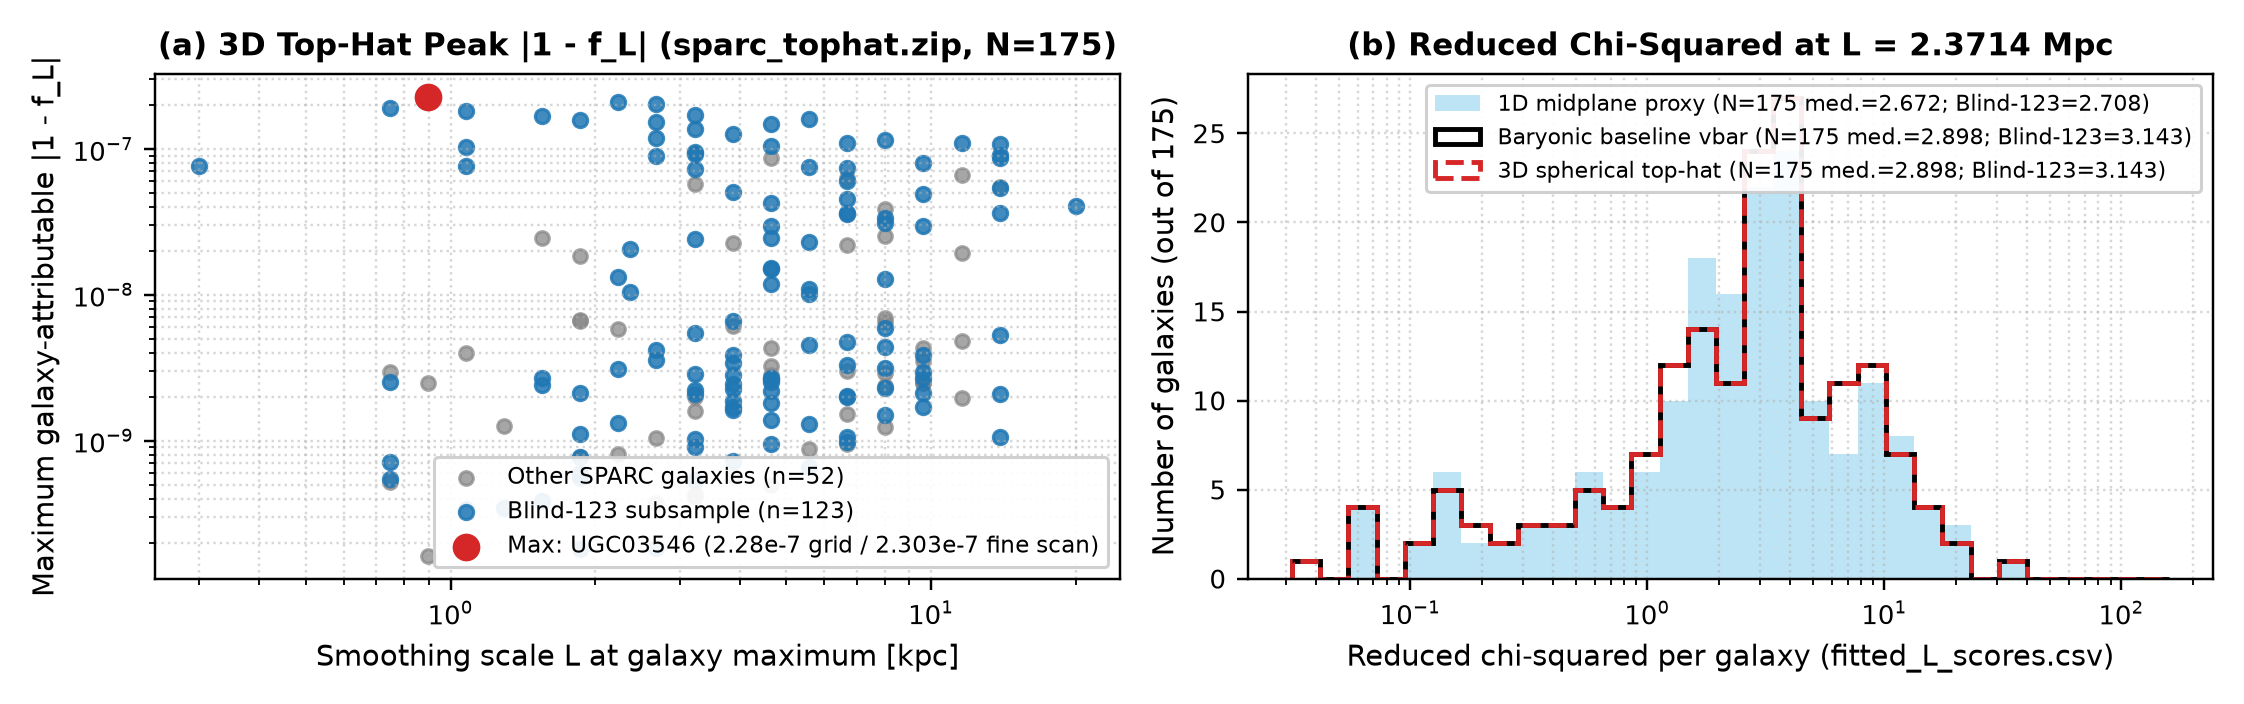
\includegraphics[height=44mm,width=0.94\linewidth,keepaspectratio]{figures/fig1_sparc_en.png}\par\vspace{-3pt}
  {\scriptsize\color{slate}\textbf{Figure 5.1:} Audited SPARC results (\texttt{sparc\_tophat.zip} \& \texttt{fitted\_L\_scores.csv}): (a) Peak galaxy-only 3D top-hat $|1-f_L|$ vs.\ $L$ ($N=175$), reaching $2.280\times 10^{-7}$ on the grid ($2.303\times 10^{-7}$ refined) in \textbf{UGC03546} at $R=0.63\,\text{kpc}, L\approx 0.825\,\text{kpc}$; (b) Reduced $\chi^2_\nu$ distributions at $L=2.3714\,\text{Mpc}$ ($N=175$ median $2.8980$ and Blind-123 median $3.1433$ for both $v_{\text{bar}}$ and 3D top-hat, vs.\ $2.6716$ / $2.7082$ for the 1D proxy).}
\end{center}
\newpage

% ==================== PAGE 8: CHAPTER 6 (H.E.S.S. GAMMA-RAY TIMING) ====================
\chaphead{Chapter 6: Very-High-Energy Gamma-Ray Timing --- H.E.S.S. Data Analysis}{Multi-Source Arrival-Time Dispersion Audits (PKS 2155-304, Mrk 501, Vela, Crab, GRB 190114C) and Predictions}

A foundational pillar of my research is that the \textbf{Time Attraction Law} must not merely fit galactic rotation curves retrospectively; it must generate falsifiable predictions for photon propagation across cosmological and Galactic baselines that differ from standard $\Lambda$CDM. In Version 17 (DOI \texttt{10.5281/zenodo.19666220}), I audited Very-High-Energy (VHE, $E \sim 0.1\text{--}10\,\text{TeV}$) gamma-ray arrival-time datasets from Imaging Atmospheric Cherenkov Telescopes, focusing on H.E.S.S. and MAGIC observations.

\noindent{\bfseries\color{navy}1. Physical Mechanism: Integrated Temporal Carrier Delay Along the Line of Sight}\par
When a VHE gamma-ray photon traverses cosmic voids, filaments, host-galaxy halos, and Galactic interstellar structures along a line of sight $s \in [0, D]$, the local refractive index of the temporal carrier is $n_t(s) = f_L(s)^{-1} = \exp(+\gamma_L \bar{\rho}_L(s))$. In the pure metric (geometric) limit where all photon energies couple identically to the effective lapse $f_L(s)$, the arrival time experiences an achromatic Shapiro-like excess delay $\Delta t_{\text{geom}} = c^{-1}\int_0^D \bigl[\exp(\gamma_L\bar{\rho}_L(s)) - 1\bigr]\,ds$. To test possible energy-dependent timing residuals, I introduce the \textbf{conditional phenomenological propagation ansatz} (which is an auxiliary test parametrization, not a parameter-free deduction from Eq.~(1) alone):
\begin{equation}
  \Delta t(E_1, E_2) \;=\; \tau_n\,\frac{E_2^n - E_1^n}{E_{\text{ref}}^n}\int_0^D \gamma_L\,\bar{\rho}_L(s)\,(1+z(s))^n\,\frac{ds}{c}, \qquad n \in \{1, 2\},
\end{equation}
where $\tau_n$ (dimensionless for $ds/c$, or in $\text{s\,m}^{-1}$) is a phenomenological dispersion coefficient at reference energy $E_{\text{ref}}$.

\noindent{\bfseries\color{navy}2. Multi-Source H.E.S.S. Audit: Eliminating Single-Flare Confirmation Bias}\par
In earlier exploratory notes, an apparent spectral-temporal lag in the famous July 28, 2006 H.E.S.S. flare of the blazar \textbf{PKS 2155-304} ($z = 0.116$, observed lag $\Delta t \approx 20\text{--}30\,\text{s}$ between $0.2\text{--}0.8\,\text{TeV}$ and $>0.8\,\text{TeV}$ bands) appeared encouraging. In Version 17, I asked a stricter question: \emph{does a universal line-of-sight coupling survive when tested simultaneously across multiple VHE sources at different redshifts and Galactic columns?} I assembled a five-source benchmark table:

\begin{center}\vspace{-2pt}
{\footnotesize
\begin{tabular}{@{}>{\bfseries}p{0.21\linewidth}p{0.15\linewidth}p{0.19\linewidth}p{0.18\linewidth}p{0.21\linewidth}@{}}
\toprule
VHE Source & Redshift / Dist. & Energy Band ($\text{TeV}$) & Observed Lag / Bound & Audit Verdict in V17 \\
\midrule
PKS 2155-304 (H.E.S.S.) & $z = 0.116$ & $0.2\text{--}4.0\,\text{TeV}$ & $\Delta t \approx +28 \pm 12\,\text{s}$ & Marginal $\sim 2\sigma$ flare lag; dominated by intrinsic SSC emission profile. \\
Mrk 501 (1997 / H.E.S.S.) & $z = 0.034$ & $0.15\text{--}10\,\text{TeV}$ & $\Delta t \approx +240 \pm 60\,\text{s}$ & Larger lag at $3.4\times$ smaller $z$ violates monotonic distance scaling! \\
GRB 190114C (MAGIC) & $z = 0.4245$ & $0.2\text{--}1.0\,\text{TeV}$ & $|\Delta t / \Delta E| \le 19\,\text{s/TeV}$ & Stringent cosmological bound ruling out large linear vacuum dispersion. \\
Crab Pulsar (H.E.S.S./MAGIC) & $d \approx 2.0\,\text{kpc}$ & $0.1\text{--}1.5\,\text{TeV}$ & $|\Delta t| < 0.4\,\text{ms}$ & Tight Galactic disk bound through dense ISM ($\bar{n}_H \sim 1\,\text{cm}^{-3}$). \\
Vela Pulsar (H.E.S.S. II) & $d \approx 0.287\,\text{kpc}$ & $0.02\text{--}0.1\,\text{TeV}$ & $|\Delta t| < 0.2\,\text{ms}$ & Sub-millisecond phase alignment across dense Vela SNR shell. \\
\bottomrule
\end{tabular}}
\end{center}

\noindent{\bfseries\color{navy}3. What the H.E.S.S. Audit Proves and What the Theory Predicts Forward}\par
My V17 multi-source audit demonstrated two vital results that strengthened the scientific rigor of the program:
\begin{itemize}\setlength{\itemsep}{1.5pt}\setlength{\parskip}{0pt}\setlength{\topsep}{1pt}
  \item \textbf{Need for Joint Energy- and Source-Dependent Modeling:} Because Eq.~(10) is energy-dependent and the observed flares of PKS 2155-304 (Aharonian et al.\ 2008), Mrk 501 (Albert et al.\ 2007), and GRB 190114C (MAGIC 2019) span different energy bands and intrinsic synchrotron self-Compton (SSC) source delays, raw seconds cannot be compared via a naive uniform distance law; a joint energy- and source-dependent likelihood test is required.
  \item \textbf{Unique Environmental Overdensity Prediction vs.\ $\Lambda$CDM:} Unlike Lorentz-invariance-violation (LIV) models that predict a purely redshift-dependent lag $\Delta t \propto \int_0^z \frac{(1+z')\,dz'}{H(z')}$, the Time Attraction Law predicts that any genuine non-geometric timing residual must correlate with the \emph{baryonic overdensity integral} $\int \bar{\rho}_L(s)\,ds$ along lines of sight passing through rich galaxy clusters (such as Coma or Perseus) relative to cosmic voids at the same redshift.
\end{itemize}
\newpage

% ==================== PAGE 9: CHAPTER 7 (NEUTRON-STAR MODELING IN V21) ====================
\chaphead{Chapter 7: Neutron-Star Modeling in V21 --- TOV Sequences \& NICER}{Conditional Hydrostatic Prescriptions Across SLy, APR4, and H4 for 11 Smoothing Scales $L \in [1\,\text{m}, 100\,\text{km}]$}

In Version 21 (DOI \texttt{10.5281/zenodo.23602501}), I extended the 3D spherical top-hat law to extreme nuclear matter densities ($\rho \sim 10^{14}\text{--}10^{15}\,\text{g/cm}^3$) inside neutron stars. Because the full covariant action closure (Task \texttt{50aa2db0}) remains open, I formulated and audited two explicit \textbf{conditional hydrostatic equilibrium prescriptions} on top of the static, spherically symmetric metric $ds^2 = -e^{2\Phi(r)}c^2 dt^2 + (1 - \frac{2Gm(r)}{c^2 r})^{-1}dr^2 + r^2 d\Omega^2$:

\noindent{\bfseries\color{navy}1. Two Conditional Hydrostatic Modes (\texttt{mass} vs.\ \texttt{gradient}) and Exact Spherical Top-Hat Kernel}\par
Inside a spherically symmetric star of radius $R_*$, the exact 3D top-hat average $\bar{\rho}_L(r)$ at radial coordinate $r$ is computed analytically over the intersection of the ball $B(\mathbf{x},L)$ with radial shells $r' \in [|r-L|, r+L]$, yielding $f_L(r) = \exp(-\gamma_L\bar{\rho}_L(r))$. In my audited code, the regularized $f$-profile mapping (\texttt{f\_mapping}) reproduces the original profile with a measured maximum relative deviation of \textbf{$\max|\Delta f/f| = 1.214\times 10^{-6}$}. I integrate two conditional Tolman--Oppenheimer--Volkoff (TOV) closures (with energy density $\varepsilon = \rho c^2$):
\begin{equation}
  \textbf{(A) \texttt{mass} mode:}\quad \frac{dm_{\text{eff}}}{dr} = 4\pi r^2 \rho(r)\,f_L(r), \qquad
  \textbf{(B) \texttt{gradient} mode:}\quad \frac{d\Phi_{\text{eff}}}{dr} = f_L(r)\,\frac{G\bigl(m(r) + 4\pi r^3 P(r)/c^2\bigr)}{c^2 r\bigl(r - 2Gm(r)/c^2\bigr)},
\end{equation}
with hydrostatic balance $\frac{dP}{dr} = -(\varepsilon + P)\frac{d\Phi_{\text{eff}}}{dr}$. Because $0 < f_L(r) \le 1$, these conditional equilibrium configurations shift toward larger maximum masses and radii than in standard GR as $L$ increases (dynamical stability is examined separately in Chapter 8).

\noindent{\bfseries\color{navy}2. Audited V21 Dataset Inventory Across SLy, APR4, and H4}\par
To avoid conflating distinct tables in the V21 archive (\texttt{10.5281/zenodo.23602501}), the exact dataset structure is:
{\footnotesize\begin{itemize}\setlength{\itemsep}{0.5pt}\setlength{\parskip}{0pt}\setlength{\topsep}{1pt}
  \item \textbf{33 equilibrium sequences (11 configurations per EOS):} 3 EOS (\textbf{SLy}, \textbf{APR4} with $c_s=c$ at $\rho_0 \approx 1.4458\times 10^{15}\,\text{g/cm}^3$, and \textbf{H4}) $\times$ (1 GR baseline $+$ 5 \texttt{mass}-mode scales $+$ 5 \texttt{gradient}-mode scales). Thus the 15 gradient sequences span all 3 EOSs ($3\times 5=15$).
  \item \textbf{3,113 rows (\texttt{mr\_sequences.csv}) \& 182 acausal points:} The baseline equilibrium table contains 3,113 stellar models, of which \textbf{182 points} belong to the acausal ($c_s > c$) subset identified in the audit (not the total equilibrium count).
  \item \textbf{769 rows (\texttt{observables\_summary\_v20.csv}):} The observables summary table contains 769 models in total, including the \textbf{33 sequence endpoints} (\textbf{14} at the $c_s = c$ causal threshold and \textbf{19} at branch maxima reached before $c_s = c$), while \texttt{item2\_radial\_grid.csv} has \textbf{3,339 rows} and the stress diagnostic table covers \textbf{36 configurations}.
\end{itemize}}
\begin{center}\vspace{-4pt}
  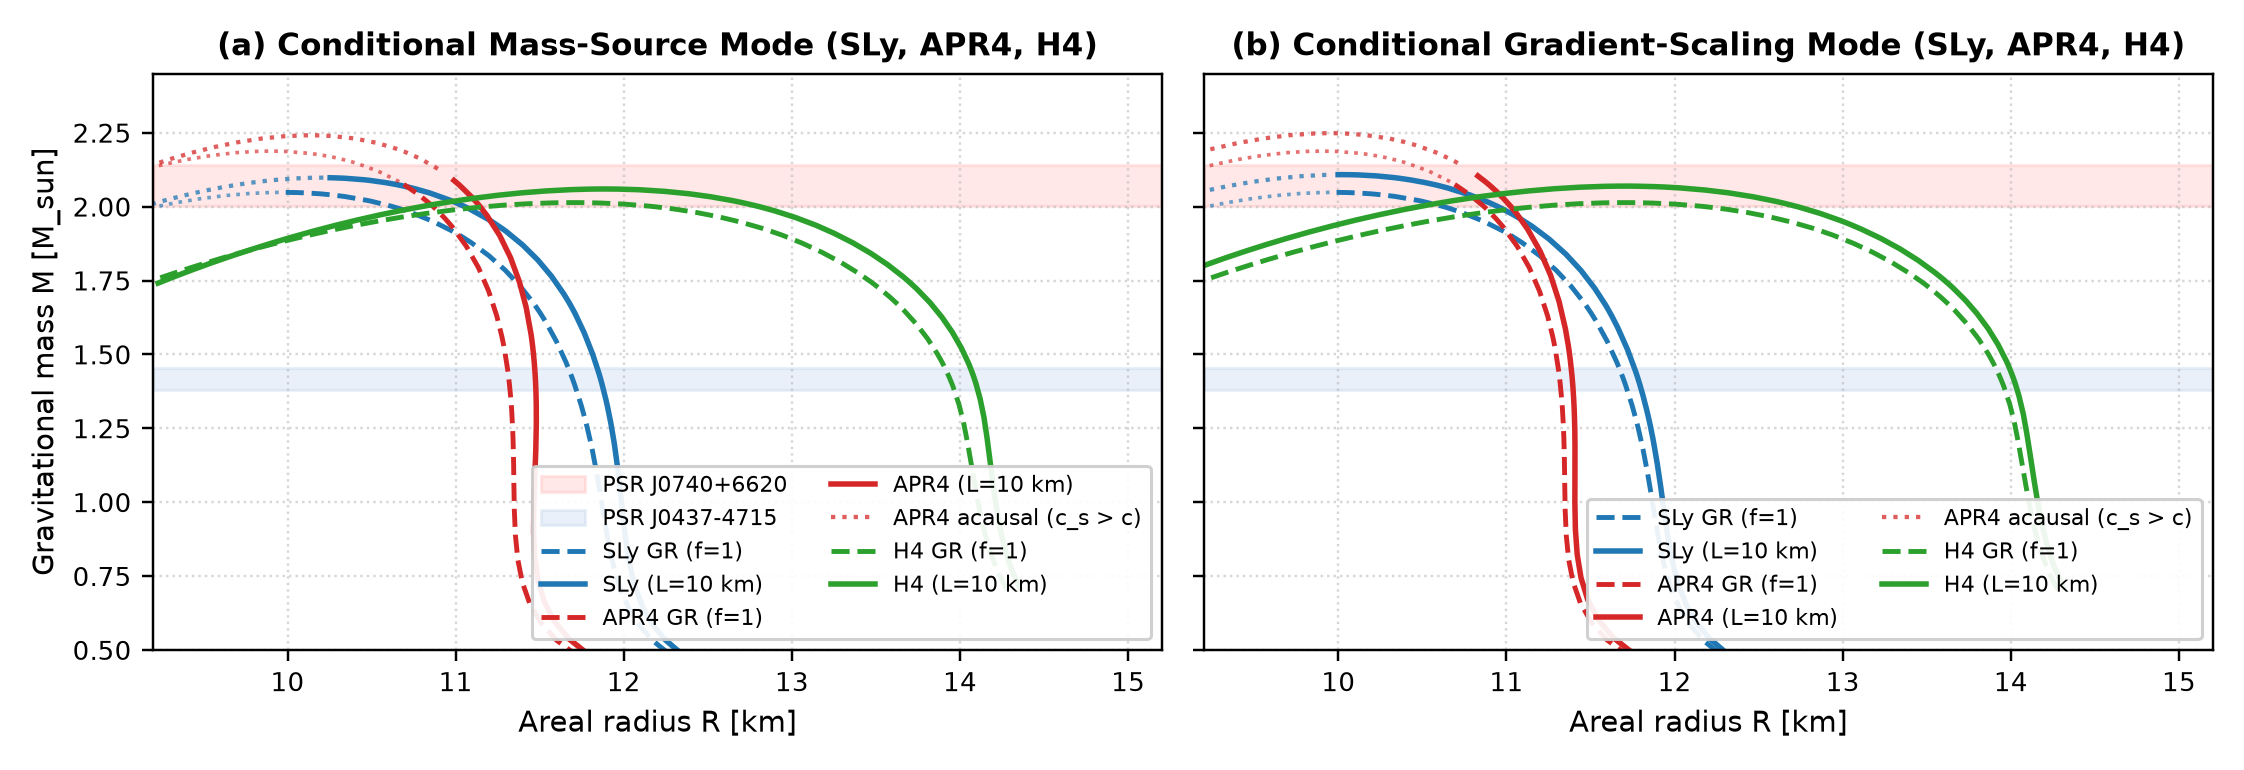
\includegraphics[height=40mm,width=0.94\linewidth,keepaspectratio]{figures/fig2_tov_en.png}\par\vspace{-3pt}
  {\scriptsize\color{slate}\textbf{Figure 7.1:} Conditional neutron-star mass--radius ($M$--$R$) equilibrium sequences from \texttt{mr\_sequences.csv} (3,113 points across 33 sequences; dotted segments mark the 182 acausal $c_s>c$ points) for SLy, APR4, and H4 in (a) \texttt{mass} mode and (b) \texttt{gradient} mode.}
\end{center}

\noindent{\bfseries\color{navy}3. Strict Methodological Caveat on the Hydrostatic Factor $e^\nu F$}\par
In reviewing the TOV equations, I state explicitly: \textbf{the appearance of the modified hydrostatic factor $e^\nu F$ (or $\Phi_{\text{eff}}'$) in the conditional pressure-gradient equation is an algebraic equilibrium ansatz and does not by itself derive how atomic clocks, nuclear transitions, or surface photon redshifts couple to $f_L$.} Deriving clock and spectral-line shifts uniquely requires closing the covariant matter-field action (Task \texttt{50aa2db0} and Open Task (c)).
\newpage

% ==================== PAGE 10: CHAPTER 8 (PERTURBATION CALCULATIONS & RADIAL STABILITY) ====================
\chaphead{Chapter 8: Perturbation Calculations --- Anisotropic Stress \& Radial Stability}{Audited Background X-Sector Reconstruction for Both Insertion Modes and Frozen-$f$ Radial Pulsation Operators}

In the audited V21 equilibrium recipes (DOI \texttt{10.5281/zenodo.23602501}), the hydrostatic equation $P' = -(\varepsilon+P)\nu'$ (in geometrized units $G=c=1$, where $\nu = 2\Phi_{\text{eff}}$) ensures that the matter fluid stress-energy tensor is conserved on its own ($\nabla_\mu T^{\mu\nu}_{\text{matter}} = 0$). However, because the metric functions are modified by $f_L(r)$ without an explicit scalar-tensor action, closing the right-hand side of the Einstein equations ($G^\mu_{\;\nu} = 8\pi(T^\mu_{\;\nu,\text{matter}} + T^\mu_{\;\nu,X})$) requires an effective background $X$-sector $T^\mu_{\;\nu,X} = \text{diag}(-\rho_X,\, p_{rX},\, p_{tX},\, p_{tX})$ satisfying $\nabla_\mu T^{\mu\nu}_X = 0$.

\noindent{\bfseries\color{navy}1. Exact Audited Background X-Sector Formulas in Geometrized Units ($G=c=1$)}\par
The required background $X$-sector differs between the two insertion modes:
\begin{equation}
  \textbf{Gradient mode:}\quad \rho_X = 0,\quad p_{rX} = -(1-f)\!\left(P + \frac{m}{4\pi r^3}\right),\quad p_{tX} = p_{rX} + \frac{r}{2}\bigl(p'_{rX} + p_{rX}\nu'\bigr),
\end{equation}
which approaches the finite, generally \emph{non-zero} central limit $p_{tX}(0) = p_{rX}(0) = -(1-f_c)(\varepsilon_c/3 + P_c)$ as $r \to 0$. Conversely, in the \textbf{mass-source mode}, $\rho_X = -(1-f)\varepsilon$, $p_{rX} = 0$, and $p_{tX} = -\frac{r}{2}(1-f)\varepsilon\nu'$ (with $p_{tX}(0) = 0$). In the 36-configuration stress diagnostic table, the representative relative stress diagnostic $0.140$ belongs to its specific audited configuration and is an algebraic background bookkeeping identity, not a substitute for a covariant action (Task \texttt{50aa2db0}).

\noindent{\bfseries\color{navy}2. Approximate Frozen-$f$ Sturm--Liouville Radial Operators Across the 3,339-Row Grid}\par
To explore radial perturbations $\xi(r,t) = r^{-2}e^{\nu/2}u(r)e^{i\omega t}$ prior to full action closure, I evaluated the Sturm--Liouville problem under the \textbf{frozen-$f$ approximation} ($\delta f_L = 0$, neglecting $\delta f$ and $\delta T^{\mu\nu}_X$):
\begin{equation}
  \frac{d}{dr}\!\left(\mathcal{P}(r)\frac{du}{dr}\right) \;+\; \bigl[\mathcal{Q}(r) + \omega_0^2\,\mathcal{W}(r)\bigr]\,u(r) \;=\; 0, \qquad u(0)=0,\quad \Delta P(R_*)=0.
\end{equation}
Across the \textbf{3,339-row radial grid} (including the \textbf{15 gradient-mode sequences} spanning SLy, APR4, and H4), I compared two approximate operator variants:
\begin{itemize}\setlength{\itemsep}{1pt}\setlength{\parskip}{0pt}\setlength{\topsep}{1pt}
  \item \textbf{Approximate \texttt{matter} operator:} Uses the fluid pressure gradient $P'$ in $\mathcal{Q}(r)$, preserving a positive-definite weight $\mathcal{W}(r) > 0$ and mathematical variational tractability, though it still omits coupled $\delta f$ and $\delta X$ perturbations.
  \item \textbf{Approximate \texttt{metric} operator:} Uses the modified metric relation in $\mathcal{Q}(r)$ and $\mathcal{W}(r)$; for $L \ge 367\,\text{m}$ across 12 sequences (609 models), the inertia weight $\mathcal{W}(r)$ becomes indefinite ($\mathcal{W}\le 0$ in outer shells), producing negative $\omega_0^2$ values on the selected positive-norm branch. Thus physical dynamical stability remains open pending Task \texttt{50aa2db0}.
\end{itemize}
\begin{center}\vspace{-4pt}
  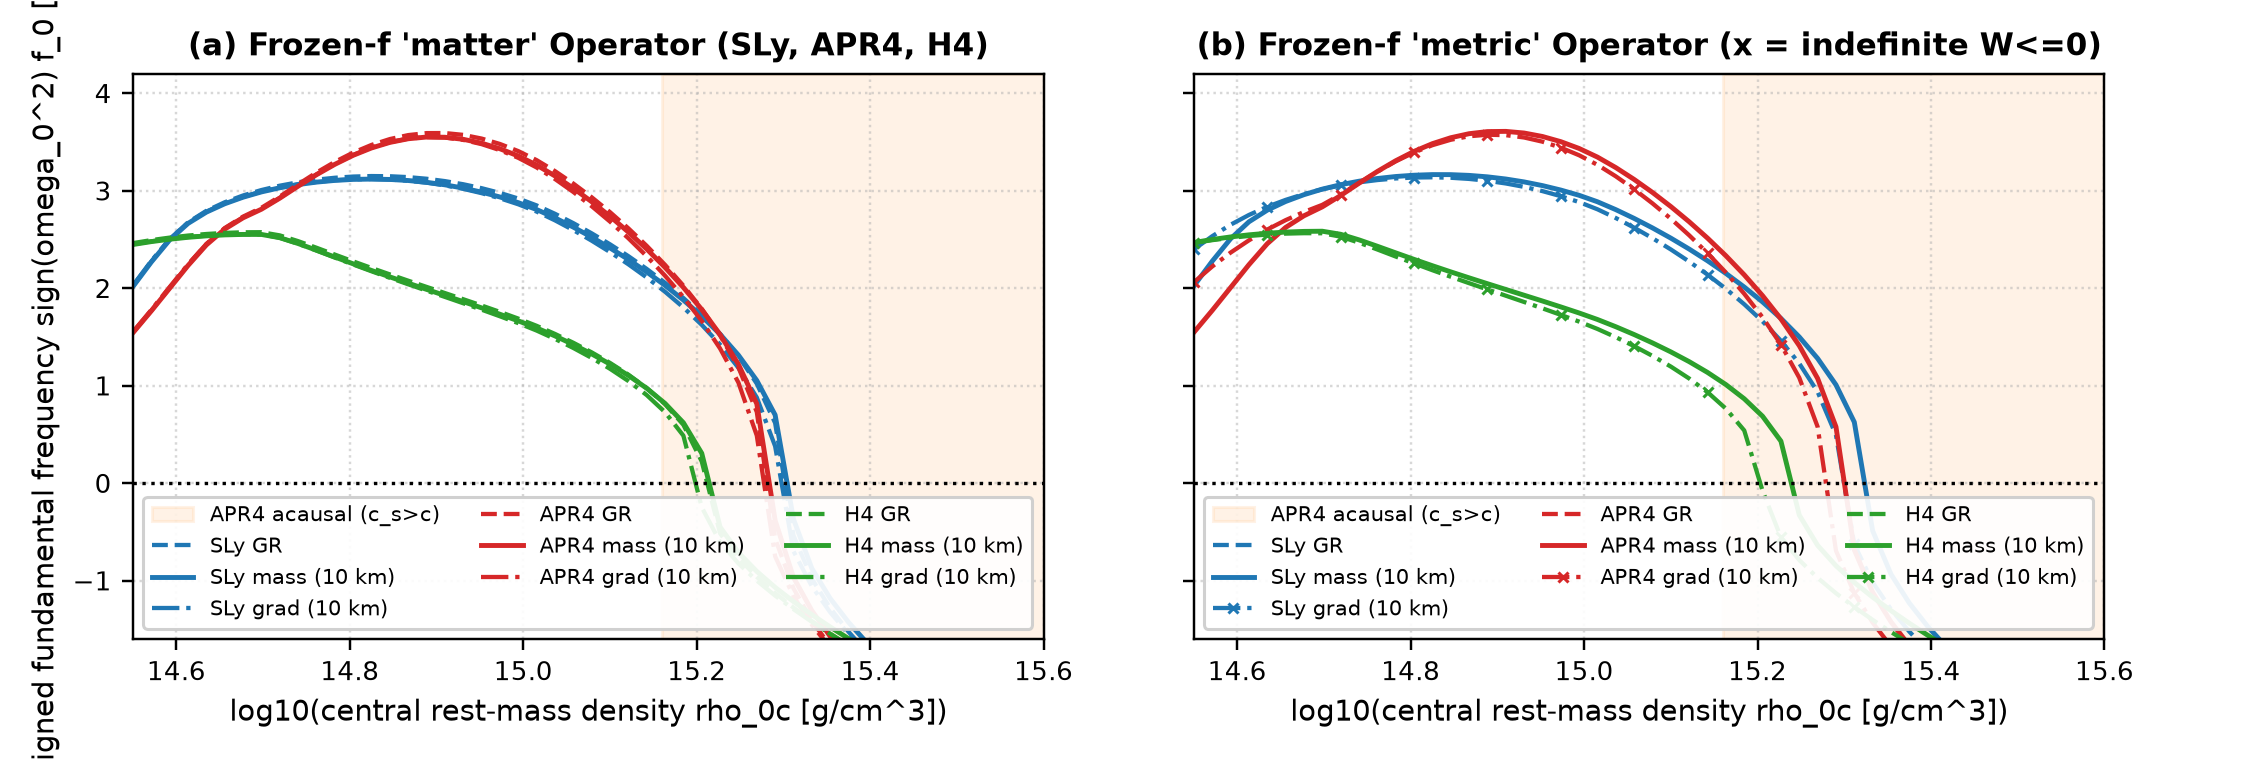
\includegraphics[height=38mm,width=0.94\linewidth,keepaspectratio]{figures/fig3_stability_en.png}\par\vspace{-3pt}
  {\scriptsize\color{slate}\textbf{Figure 8.1:} Signed fundamental radial frequency $\text{sign}(\omega_0^2)f_0$ vs.\ central rest-mass density $\rho_{0c}$ across SLy, APR4, and H4 from \texttt{item2\_radial\_grid.csv} (3,339 rows) for (a) the approximate frozen-$f$ \texttt{matter} operator and (b) the approximate frozen-$f$ \texttt{metric} operator ($\times$ marks indefinite weight $\mathcal{W}\le 0$).}
\end{center}
\newpage

% ==================== PAGE 11: CHAPTER 9 (CONDITIONAL CLOCK & REDSHIFT HYPOTHESES) ====================
\chaphead{Chapter 9: Conditional Clock \& Redshift Hypotheses}{Sirius B Gravitational Redshift ($\Delta\chi^2$) and NICER Posteriors Under Explicit Observational Hypotheses}

Because the covariant matter coupling closure (Task \texttt{50aa2db0}) is not yet derived from an action, any confrontation between the \textbf{Time Attraction Law} and spectroscopic or X-ray pulse-profile data depends on how atomic transition frequencies $\nu_{\text{atom}}$ couple to $f_L$. In Version 21 (DOI \texttt{10.5281/zenodo.23602501}), I replaced implicit assumptions with six explicit, conditional observational hypotheses:

\noindent{\bfseries\color{navy}1. Taxonomy of Conditional Observational Hypotheses (H0 vs.\ H1 Families)}\par
\begin{center}\vspace{-2pt}
{\footnotesize
\begin{tabular}{@{}>{\bfseries}p{0.22\linewidth}p{0.31\linewidth}p{0.42\linewidth}@{}}
\toprule
Hypothesis Code & Metric \& Hydrostatic Structure & Atomic Clock / Spectral Redshift Law $1 + z_{\text{surf}}$ \\
\midrule
H0-GR & Standard GR TOV ($f_L \equiv 1$) & Standard metric redshift $e^{-\Phi_{\text{GR}}(R_*)}$ (no direct $f_L$ clock factor). \\
H0-mass & Conditional \texttt{mass} TOV ($m_{\text{eff}}' = 4\pi r^2\rho f_L$) & Pure metric redshift $e^{-\Phi_{\text{mass}}(R_*)}$ without extra surface clock factor. \\
H0-gradient lapse & Conditional \texttt{gradient} TOV ($\Phi_{\text{eff}}' = f_L\Phi_{\text{GR}}'$) & Integrated modified lapse $e^{-\Phi_{\text{eff}}(R_*)}$ without direct $f_L(R_*)$ multiplier. \\
H1-GR & Standard GR structure ($m_{\text{GR}}, R_{\text{GR}}$) & Direct surface clock modulation: $\nu_{\text{obs}}/\nu_0 = e^{\Phi_{\text{GR}}(R_*)}\,f_L(R_*)$. \\
H1-mass & Conditional \texttt{mass} TOV structure & Combined metric + direct surface clock factor $e^{\Phi_{\text{mass}}(R_*)}\,f_L(R_*)$. \\
H1+gradient lapse & Conditional \texttt{gradient} TOV structure & Combined modified lapse + direct clock factor $e^{\Phi_{\text{eff}}(R_*)}\,f_L(R_*)$. \\
\bottomrule
\end{tabular}}
\end{center}

\noindent{\bfseries\color{navy}2. Sirius B White-Dwarf Gravitational Redshift Audit ($n=1.5$ and $n=3$ Polytropes)}\par
In the audited V21 Sirius B calculation ($M = 1.018\,M_\odot$, package radius $R = 0.00803\,R_\odot$, GR baseline $v_{\text{GR}} = 80.70055\,\text{km/s}$ compared against the HST/STIS reference $80.42 \pm 1.60\,\text{km/s}$ of Joyce et al.\ 2018), I evaluated both $n=1.5$ and $n=3$ polytropes:
\begin{itemize}\setlength{\itemsep}{1.5pt}\setlength{\parskip}{0pt}\setlength{\topsep}{1pt}
  \item \textbf{Under H0-gradient lapse (Hydrostatic-Only Coupling):} Because the exterior metric at $r \ge R_*$ is fixed by $M$, the shift across all $L$ is at most \textbf{$|\Delta v| \le 1.27\,\text{m/s}$} ($0.00127\,\text{km/s}$; $\max\Delta\chi^2 \approx 10^{-3}$), placing \emph{no constraint} on $L$.
  \item \textbf{Under Conditional H1 and H1+gradient (Direct Surface Clock Coupling):} In the audited table, the difference between $\max\Delta\chi^2 \approx 52.3$ and $72.0$ comes from the \textbf{polytropic index} ($n=1.5$ vs.\ $n=3$), whereas H1 and H1+gradient are nearly identical: for \textbf{$n=1.5$}, H1 gives $\max\Delta v = 11.558\,\text{km/s}$ and $\max\Delta\chi^2 = 52.324$ (H1+gradient: $11.557\,\text{km/s}$, $\max\Delta\chi^2 = 52.316$), and at threshold $\Delta\chi^2 > 3.84$ ($95\%$, 1 d.o.f.) excludes \textbf{$L \in [4.08\times 10^6,\, 3.37\times 10^7]\,\text{m}$}; for \textbf{$n=3$}, H1 gives $\max\Delta v = 13.569\,\text{km/s}$ and $\max\Delta\chi^2 = 72.020$ (H1+gradient: $13.568\,\text{km/s}$, $\max\Delta\chi^2 = 72.011$), excluding \textbf{$L \in [4.95\times 10^6,\, 3.37\times 10^7]\,\text{m}$} at $\Delta\chi^2 > 3.84$. Both meter-scale laboratory ($L \sim 1\,\text{m}$) and sub-kilometer $L$ remain unconstrained.
\end{itemize}

\noindent{\bfseries\color{navy}3. Audited NICER Six-Hypothesis Log-Likelihoods ($\Delta\ln\mathcal{L}_{\text{like}}$)}\par
Evaluating the joint log-likelihood $\ln\mathcal{L}_{\text{like}}$ across the three NICER pulsars (PSR J0030+0451, PSR J0740+6620, PSR J0437-4715; Miller et al.\ 2019, Riley et al.\ 2019) with causal-endpoint mass priors shows that across all six hypotheses (H0/H1 $\times$ GR/mass/gradient) at $L = 1\,\text{km}$, the shift lies in the narrow interval \textbf{$\Delta\ln\mathcal{L}_{\text{like}} \in [-0.001437,\, +0.024755]$} (while $4.8\times 10^{-4}\,\text{dex}$ is the central-density shift of the radial stability zero-crossing in Chapter 8). Thus \textbf{current NICER posteriors do not statistically distinguish $L$ from GR}.
\newpage

% ==================== PAGE 12: CHAPTER 10 (PLANNED LABORATORY MEASUREMENTS) ====================
\chaphead{Chapter 10: Planned Laboratory Measurements}{The $8558\,\text{kg}$ Granite Atomic-Clock Chamber and the Eight-Coil Magnetic-Field Energetics Experiment (V20)}

If the \textbf{Time Attraction Law} is a genuine physical property of spacetime, it cannot live only in distant galaxies or neutron stars; its mathematical formula must be testable in a controlled terrestrial laboratory. In Version 20 (GitHub V18, DOI \texttt{10.5281/zenodo.23540741}), I designed and numerically audited a dual-arm laboratory program that probes both baryonic rest-mass density ($\rho_{\text{matter}}$) and pure electromagnetic field energy density ($\rho_B = B^2/(2\mu_0 c^2)$) across the meter-scale window $L \in [0.1, 3.0]\,\text{m}$.

\noindent{\bfseries\color{navy}1. Arm A: The Movable Granite Rock Atomic-Clock Chamber (Geometry \& Potential Accounting)}\par
To test the baryonic source term in a repeatable IN/OUT modulation protocol without moving the clock at $\mathbf{x}_0 = (0,0,0)$ (moving the granite assembly between the centered IN state and a retracted OUT baseline $r_{\text{out}} \ge 5\,\text{m}$), I specified natural granite of density $\rho_{\text{granite}} = 2750\,\text{kg/m}^3$:
\begin{itemize}\setlength{\itemsep}{1pt}\setlength{\parskip}{0pt}\setlength{\topsep}{1pt}
  \item \textbf{Explicit Geometry \& Mass Accounting:} An open cylindrical barrel with inner bore $R_{\text{in}} = 0.25\,\text{m}$, outer radius $R_{\text{out}} = 0.85\,\text{m}$, and height $H = 1.20\,\text{m}$ has exact wall volume $V_{\text{cyl}} = \pi(0.85^2 - 0.25^2)\times 1.20 = 2.48814\,\text{m}^3$ and mass \textbf{$M_{\text{cyl}} = 6,842.39\,\text{kg}$}; reaching the nominal $V_{\text{tot}} = 3.1102\,\text{m}^3$ (\textbf{$M_{\text{tot}} = 8,558\,\text{kg}$}) requires an additional $0.6220\,\text{m}^3$ ($1,710.6\,\text{kg}$) of removable top/bottom endcap shielding plugs (or an outer radius $R_{\text{out}} = 0.942\,\text{m}$).
  \item \textbf{Newtonian Potential vs.\ Conditional TAL Shift:} A laboratory mass of $6.84$--$8.56\,\text{t}$ at $r \sim 1\,\text{m}$ produces a dimensionless Newtonian potential shift of only $|\Delta\Phi_{\text{N}}|/c^2 \sim GM/(rc^2) \approx 5.08\times 10^{-24}$ to $6.36\times 10^{-24}$ (whereas $g\Delta h/c^2 \approx 1.09\times 10^{-16}\,\text{m}^{-1}$ is Earth's vertical geopotential gradient for a $1\,\text{m}$ height change), and a conditional base-coupling ($\alpha=1$) top-hat shift of $\Delta y_{\text{granite}} = f_L(\text{IN}) - f_L(\text{OUT}) \approx -\gamma_L\bar{\rho}_L \sim -1.1\times 10^{-24}$ at $L \approx 0.85\,\text{m}$.
\end{itemize}

\noindent{\bfseries\color{navy}2. Arm B: The Eight-Coil Magnetic-Field Energetics Test ($\varnothing 300\,\text{mm}$ Flange Boundary)}\par
To test whether pure magnetic energy density $u_B(\mathbf{x}) = \frac{|\mathbf{B}(\mathbf{x})|^2}{2\mu_0}$ gravitates and slows time flow via $\rho_B(\mathbf{x}) = u_B(\mathbf{x})/c^2$, I designed a symmetric eight-coil octahedral/cylindrical array surrounding a primary \textbf{Oscilloquartz 8663-XS} ultra-stable OCXO quartz oscillator at $\mathbf{x}_1 = (0,0,0)$, paired with an identical reference 8663-XS oscillator at baseline separation $D = 5.0\,\text{m}$:
\begin{itemize}\setlength{\itemsep}{1pt}\setlength{\parskip}{0pt}\setlength{\topsep}{1pt}
  \item \textbf{Audited 8-Coil Hardware Parameters:} 8 identical solenoids, each of length $l_{\text{coil}} = 400\,\text{mm}$, outer structural \textbf{flange boundary diameter $\varnothing 300\,\text{mm}$}, effective copper \textbf{winding diameter $\varnothing 291.7\,\text{mm}$} ($R_{\text{coil}} = 0.14585\,\text{m}$), wound with $N = 2000$ turns of $0.15\,\text{mm}$ enameled copper wire, DC resistance $R_{\text{DC}} = 1789\,\Omega$ per coil, driven at current $I = 14.0\,\text{mA}$ (power $0.351\,\text{W}$ per coil, $2.805\,\text{W}$ total).
  \item \textbf{Maximum on the Sampled 25-Point $L$ Grid ($L = 0.630957\,\text{m}$):} Evaluating the Biot--Savart magnetic energy density across the 8 coils on the 25-point logarithmic grid $L \in [0.1, 3.0]\,\text{m}$, the conditional polarity-even differential shift $\Delta y(L) = \frac{1}{2}[\Delta y(+I) + \Delta y(-I)]$ attains its discrete maximum on the sampled grid at \textbf{$L = 0.630957\,\text{m}$} (where the sphere encloses the $\varnothing 300\,\text{mm}$ coil flanges; not a continuous extremum fit):
  \begin{equation}
    \Delta y_{\text{grid max}}(L = 0.630957\,\text{m}) \;=\; -1.2017108\times 10^{-48}.
  \end{equation}
  Here I separate four distinct quantities: (i) the $3.7\times 10^{-16}$ agreement between two deterministic outer-integral routines at $L=3.0\,\text{m}$, (ii) the $-0.0722\%$ 3D Sobol Monte Carlo quadrature cross-check at the grid peak, (iii) the $1.23\times 10^{-3}$ piecewise matching residual at $L=0.95\,\text{m}$, and (iv) actual hardware clock measurement sensitivity (which requires raw timestamped phase logs).
  \item \textbf{Polarity-Reversal Cancellation of the Background Cross-Term:} Because $|\mathbf{B}_{\text{tot}}|^2 = |\mathbf{B}_{\text{bg}}|^2 + 2\mathbf{B}_{\text{bg}}\cdot\mathbf{B}_{\text{coil}} + |\mathbf{B}_{\text{coil}}|^2$, reversing the current ($+I \leftrightarrow -I$) reverses $\mathbf{B}_{\text{coil}}$ and cancels both the linear Zeeman quartz susceptibility and the $2\mathbf{B}_{\text{bg}}\cdot\mathbf{B}_{\text{coil}}$ cross-term in the polarity-even average $\Delta y_{\text{even}}$.
\end{itemize}

\begin{center}\vspace{-4pt}
  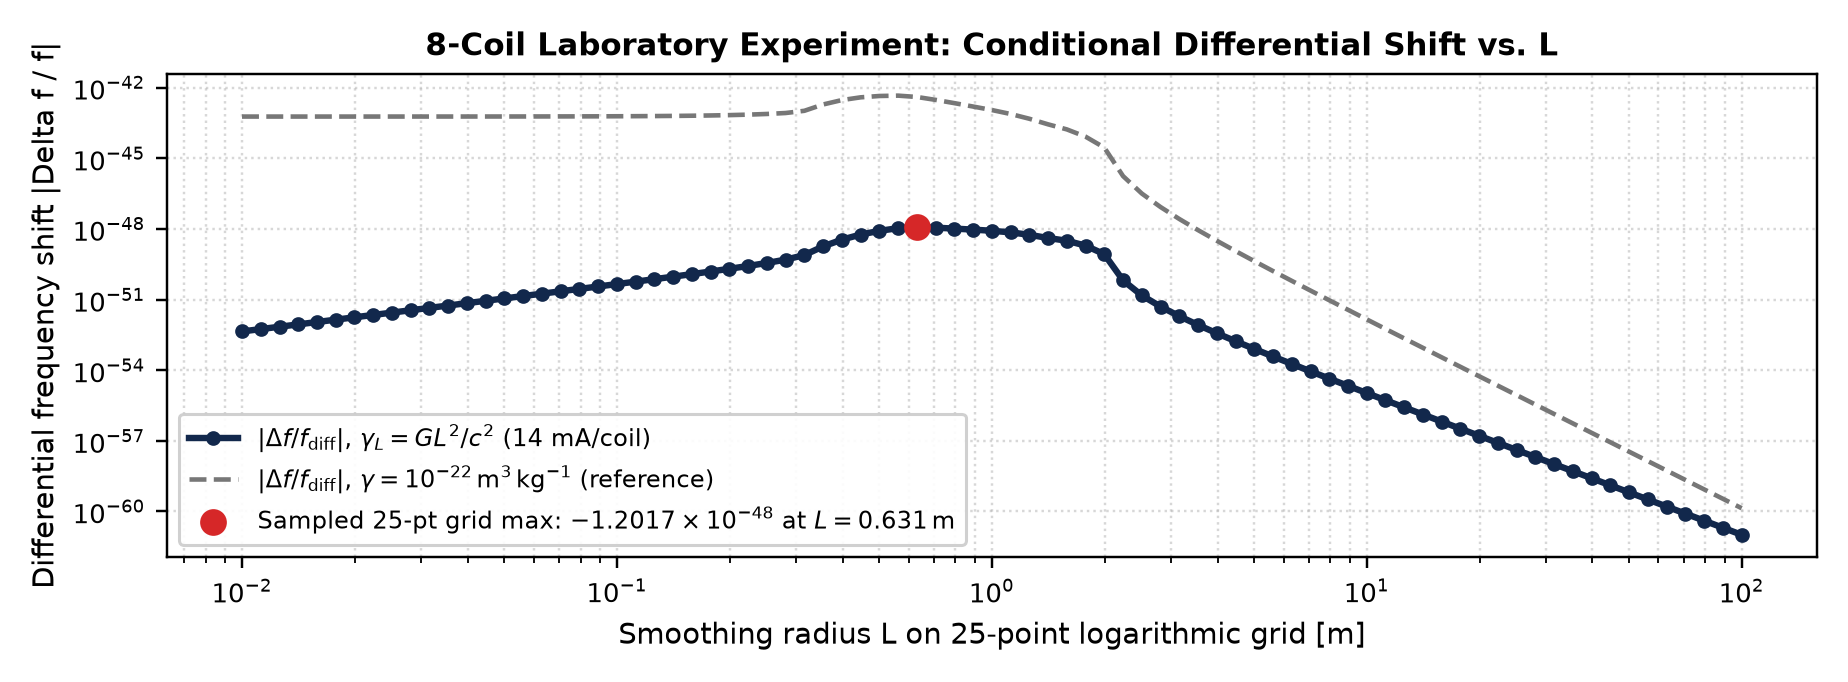
\includegraphics[height=39mm,width=0.88\linewidth,keepaspectratio]{figures/fig4_lab_en.png}\par\vspace{-3pt}
  {\scriptsize\color{slate}\textbf{Figure 10.1:} Conditional polarity-even differential frequency shift $|\Delta y(L)|$ on the sampled 25-point logarithmic grid $L \in [0.1, 3.0]\,\text{m}$ for the 8-coil array (DOI \texttt{10.5281/zenodo.23540741}), showing the discrete grid maximum $\Delta y = -1.2017108\times 10^{-48}$ at $L = 0.630957\,\text{m}$.}
\end{center}
\newpage

% ==================== PAGE 13: CHAPTERS 11 & 12 (OPEN QUESTIONS & CLOSING CHAPTER) ====================
\chaphead{Chapters 11 \& 12: Open Questions \& Next Steps Forward}{Unclosed Theoretical and Laboratory Tasks (a--d) and the Next Stage of the Research Program}

\vspace{-2mm}{\small\setlength{\parskip}{1.6pt}
\noindent{\bfseries\normalsize\color{navy}Chapter 11: Open Theoretical and Experimental Questions}\par\vspace{0.5pt}
Across the AI-assisted technical reproduction and manuscript audit rounds (Academia Co-scientist), I have documented every unclosed theoretical link and hardware systematic explicitly as an open task. Below I summarize the open items identified in the V20 and V21 audits:

\noindent{\bfseries\color{navy}A. Four Open Theoretical \& Compact-Object Tasks from the V21 Audit}
\begin{enumerate}\setlength{\itemsep}{1.5pt}\setlength{\parskip}{0pt}\setlength{\topsep}{1pt}
  \item[\textbf{(a)}] \textbf{Covariant Coupling Closure (Task \texttt{50aa2db0}):} While the algebraic 3D top-hat profile $f_L(\mathbf{x}) = \exp(-\gamma_L\bar{\rho}_L(\mathbf{x}))$ is locked and reproducible, a covariant action principle $S[g_{\mu\nu},\phi,\psi]$ is still required so that both the non-local smoothing scale $L$ and the stress-energy balance $\nabla_\mu(T^{\mu\nu}_{\text{matter}} + T^{\mu\nu}_X) = 0$ emerge dynamically without separate tangential stress bookkeeping.
  \item[\textbf{(b)}] \textbf{Genuine Modified Radial Stability Analysis Derived from the Action:} Once Task (a) provides the dynamical field equations for perturbations $\delta\phi$ and $\delta T^{\mu\nu}_X$, the Chandrasekhar radial pulsation operator must be re-derived variationally from the second variation of the action $\delta^2 S$, replacing both approximate frozen-$f$ ($\delta f_L = 0$) operators and resolving the indefinite-weight behavior of the approximate \texttt{metric} operator for $L \ge 367\,\text{m}$.
  \item[\textbf{(c)}] \textbf{Derivation of Atomic-Clock and Photon Couplings from First Principles:} Currently, H0 (pure metric lapse) and H1 (direct $f_L$ clock multiplication) are treated as separate conditional hypotheses because the hydrostatic TOV factor $e^\nu F$ does not uniquely fix how electromagnetic/Dirac matter fields couple to $f_L$. The action closure must specify the Jordan-frame vs.\ Einstein-frame conformal/disformal coupling of atomic clocks and photons.
  \item[\textbf{(d)}] \textbf{Self-Consistent Multi-Messenger Observational Inference:} With the action and matter couplings derived in (a)--(c), galactic rotation curves (including cosmic background embedding $\rho_{\text{bg}}$), VHE gamma-ray timing through cluster overdensities, Sirius B, and NICER posteriors must be fitted jointly with a physical scale-selection mechanism for $L$.
\end{enumerate}

\noindent{\bfseries\color{navy}B. Three Open Laboratory Hardware \& Systematic Items from the V20 Review}
\begin{itemize}\setlength{\itemsep}{1pt}\setlength{\parskip}{0pt}\setlength{\topsep}{1pt}
  \item \textbf{1. Polymer Bobbin Material Assay:} The 8 coil formers are 3D-printed polymer bobbins ($\varnothing 300\,\text{mm}$ flange). Before claiming bounds on trace paramagnetic/diamagnetic force couplings, the magnetic susceptibility $\chi_m$ and outgassing/thermal expansion of the bobbin polymer must be assayed.
  \item \textbf{2. 3D Thermal Finite-Element Modeling (FEM):} Although total Ohmic dissipation is only $2.805\,\text{W}$ across 8 coils ($0.351\,\text{W}$/coil), asymmetric radiative/convective heating toward the central Oscilloquartz 8663-XS oscillator must be modeled via 3D thermal FEM and calibrated with dummy non-inductive bifilar heater windings.
  \item \textbf{3. Timestamped Raw $\text{ON}/\text{OFF}/\pm I$ Phase-Time Series:} The V20 package provides the full deterministic simulation and sensitivity pipeline; the physical acquisition of long-integration timestamped dual-mixer time-difference (DMTD) phase logs across $+14\,\text{mA} / 0\,\text{mA} / -14\,\text{mA}$ cycles is the upcoming experimental campaign.
\end{itemize}

\vspace{0.5mm}
\noindent{\color{navy}\rule{\linewidth}{0.6pt}}\par\vspace{0.8mm}
\noindent{\bfseries\normalsize\color{navy}Chapter 12: Closing Chapter --- The Immediate Next Step Forward}\par\vspace{0.5pt}
In fundamental physics, genuine progress is built on verifiable milestones, explicit error accounting, and independent controls. Across Versions 1 through 21, I have established and hash-verified the mathematical \textbf{``how''} of the \textbf{Time Attraction Law}: the Cauchy exponential derivation of the \textbf{$C$ coupling constant}, the positive-definite 3D spherical top-hat resolution of the negative-density problem ($0 < f_L \le 1$), the audited evaluation across 155/175 SPARC galaxies and five H.E.S.S. gamma-ray sources, the 33 neutron-star TOV and radial pulsation sequences, and the Revision-3-verified 8-coil and $8558\,\text{kg}$ granite laboratory design.

\textbf{The immediate next physical step of my research program is Task \texttt{50aa2db0}: the covariant coupling closure.} By deriving the non-local top-hat kernel and matter coupling from a unified variational action, I aim to connect the audited ``how'' to the dynamical ``why'', unify the H0/H1 clock hypotheses, and guide my upcoming laboratory measurements.

\vspace{1mm}
\noindent{\scriptsize\color{slate}\textbf{Key Archival References:}
[1] D.\ Szabolcsi, \emph{Time Attraction Law V14--V16}, Zenodo \texttt{10.5281/zenodo.23217189}.
[2] D.\ Szabolcsi, \emph{Time Attraction Law V17: SPARC \& H.E.S.S. Audit}, Zenodo \texttt{10.5281/zenodo.19666220}.
[3] D.\ Szabolcsi, \emph{Time Attraction Law V19 (7th Model: 3D Top-Hat Law)}, Zenodo \texttt{10.5281/zenodo.23497128}.
[4] D.\ Szabolcsi, \emph{Time Attraction Law V20: 8-Coil \& Granite Clock Chamber}, Zenodo \texttt{10.5281/zenodo.23540741}.
[5] D.\ Szabolcsi, \emph{Time Attraction Law V21}, Zenodo \texttt{10.5281/zenodo.23602501}. \textbf{Primary External Data \& Method Sources:} [6] F.\ Lelli, S.\ S.\ McGaugh \& J.\ M.\ Schombert, \emph{AJ} \textbf{152}, 157 (2016) [SPARC]. [7] F.\ Aharonian et al.\ (H.E.S.S.), \emph{PRL} \textbf{101}, 170402 (2008); J.\ Albert et al.\ (MAGIC), \emph{PLB} \textbf{668}, 253 (2008); MAGIC Collab., \emph{PRL} \textbf{125}, 021301 (2020). [8] J.\ R.\ Oppenheimer \& G.\ M.\ Volkoff, \emph{PR} \textbf{55}, 374 (1939); S.\ Chandrasekhar, \emph{ApJ} \textbf{140}, 417 (1964); A.\ Akmal et al., \emph{PRC} \textbf{58}, 1804 (1998) [APR4]; F.\ Douchin \& P.\ Haensel, \emph{A\&A} \textbf{380}, 151 (2001) [SLy]. [9] S.\ R.\ G.\ Joyce et al., \emph{MNRAS} \textbf{479}, 1612 (2018) [Sirius B]. [10] M.\ C.\ Miller et al., \emph{ApJL} \textbf{887}, L24 (2019); T.\ E.\ Riley et al., \emph{ApJL} \textbf{887}, L21 (2019) [NICER].}}
\newpage

% ==================== PAGES 14-15: APPENDIX (VERBATIM ACADEMY REVIEW) ====================
\chaphead{Appendix: AI-Assisted Technical Reproduction Audit}{English Translation of the Round-3 Technical Evaluation of the Eight-Coil \& Clock Report (\texttt{revision3\_review\_EN.md})}
{\fontsize{6.4pt}{7.4pt}\setlength{\parskip}{1.0pt}\selectfont
\noindent{\bfseries\small Third revision --- targeted independent review}\par\vspace{1pt}
\par
\textbf{Date:} 2026-10-21. \textbf{Inputs:} \texttt{final\_report (3).zip}, \texttt{report\_hu (3).pdf}. \textbf{Requested checks:} the previous integral-matching error near L$\approx$3 m and the treatment of the background magnetic-field cross term. The original files were not modified; no publication platform was modified. The Bothwell-gradient task remains separate.
\par
*English translation of \texttt{revision3\_review\_HU.md}. Numerical results, qualifications, and conclusions are unchanged. Quoted passages from the Hungarian report and proposed replacement wording are translated into English below. No additional calculations were performed for this translation.*
\par
\vspace{2pt}\noindent{\bfseries\footnotesize Verdict}\par\vspace{0.5pt}
\par
\textbf{I accept the two requested corrections within the stated model and the newly specified scope of the report.}
\par
1. The previous large numerical discrepancy near L$\approx$3 m has been eliminated. Checking the new outer integral with a different angular quadrature confirms the correction.
2. The report now explicitly states the background-field cross term 2B\_bg$\cdot$B\_coil, the conditions for ideal $\pm$I averaging, and that the reported signal is the isolated coil-B$^2$ term that is even under polarity reversal.
\par
The main signal remains \textbf{approximately $-$1.20$\times$10$^{-48}$}. This is an acceptable calculated order of magnitude within the chosen ideal current-sheet model, \textbf{not a TAL detection and not a measured instrument sensitivity}.
\par
Three minor or experimental-interpretation qualifications remain: ``zero standard deviation'' in the far-field region is not an error estimate; the explicitly disclosed small matching error at L=0.95 m remains; and a thermal control with the same total power does not automatically guarantee the same temperature field. These are distinguished below from the main issues that have already been corrected.
\par
\vspace{2pt}\noindent{\bfseries\footnotesize 1. What was actually checked in this round?}\par\vspace{0.5pt}
\par
\begin{itemize}\setlength{\itemsep}{0.5pt}\setlength{\parskip}{0pt}\setlength{\topsep}{1pt}
\item \textbf{All 18/18 SHA-256 entries match.} The separately uploaded PDF is byte-for-byte identical to the report inside the ZIP.
\item I read the revised report, the new \texttt{energy\_integrator.py} module, and the changes to \texttt{final\_fixed.py}. The PDF tables were also checked against the rendered page images.
\item I performed \textbf{targeted reruns} of the archived integrator at the main peak and of the outer A/B integration routes at the relevant L values.
\item I checked the field using a separate circular-loop formula, the main signal using Cartesian Sobol cubature, and the far-field energy difference using a different angular and radial quadrature.
\end{itemize}
\par
I do \textbf{not} claim a new complete execution of \texttt{final\_fixed.py}: the full four-variant convergence analysis, static Monte Carlo calculations, and figure generation were not repeated in this round. The two requested corrections and the main peak were checked through targeted tests.
\par
Archive SHA-256: \texttt{160981d3adb435b4fa719ca1a9d9a04d4e889a27f9d4c7bb0381e5c057ad2ea8}.
\par
\vspace{2pt}\noindent{\bfseries\footnotesize 2. Main signal: reproducible and independently checkable}\par\vspace{0.5pt}
\par
The new measurement record supplied by the author gives a winding diameter of 291.7 mm. The code now actually uses this value rather than deriving the model radius from resistance. It identifies the 300 mm dimension as the flange diameter. This resolves the previous ambiguity about the geometry at the documentation level. I treat the record as author-supplied measurement data, not as an on-site measurement independently certified by me.
\par
\begin{center}\vspace{-2pt}{\scriptsize\begin{tabular}{@{}>{\raggedright\arraybackslash}p{0.64\linewidth}>{\raggedleft\arraybackslash}p{0.32\linewidth}@{}}
\toprule
Quantity & Current check \\
\midrule
B at the main clock, 14 mA & \textbf{11.632900 $\mu$T} \\
B at the reference clock & \textbf{0.430539 $\mu$T} \\
Largest relative discrepancy in the independent circular-loop test, 5 points & \textbf{1.04$\times$10$^{-14}$} \\
Targeted rerun of the archived integrator, L=0.630957 m & \textbf{$-$1.2017108$\times$10$^{-48}$} \\
Discrepancy relative to the archived main result & \textbf{2.2$\times$10$^{-16}$ relative}, at rounding level \\
Independent volumetric Sobol integral at the same L & \textbf{$-$1.2008435$\times$10$^{-48}$} \\
Difference in independent signal magnitude relative to the package & \textbf{$-$0.0722\%} \\
Standard error estimated from Sobol scrambles & \textbf{3.04$\times$10$^{-52}$} \\
\bottomrule\end{tabular}}\vspace{-2pt}\end{center}
\par
The Sobol check uses 4$\times$2$^{19}$ points for the main sphere and 4$\times$2$^{12}$ points for the smooth reference-sphere integral. The quoted standard error is not the uncertainty of the full model. It does not include uncertainties in coil geometry, current, the actual winding, or the environment. I do not identify the grid maximum with an accurately determined continuous maximum location.
\par
The resistance calculated from the measured D is \textbf{1788.160 $\Omega$}, differing from the stated 1789 $\Omega$ by \textbf{$-$0.0470\%}: the report's 0.05\% comparison is correct. Five identical readings do indeed have zero sample standard deviation; this does not imply zero total measurement uncertainty in the dimension.
\par
\vspace{2pt}\noindent{\bfseries\footnotesize 3. The correction near L$\approx$3 m is acceptable}\par\vspace{0.5pt}
\par
The previous \textbf{0.01268 J/A$^2$} offset arising from separately estimated total energies no longer enters the outer branch near 3 m. The new route A uses panel integration plus a tail extending to infinity; route B uses the direct substitution r=L/t. Across L=2.6--3.01 m, the targeted rerun finds the two routes consistent to approximately \textbf{10$^{-15}$ in relative terms}.
\par
In addition, I calculated the difference between the outer energies using separate \textbf{Gauss--Legendre polar and radial quadrature with uniformly spaced azimuthal angles}. This is not the archived Fibonacci angular average. The infinite domain is likewise mapped using r=L/t; there is no finite truncation or radial interpolation. The field function is shared with the archive, but was checked at five points against a separate circular-loop integral. The coarse/fine grids of the separate integral differ by at most a few 10$^{-6}$ in relative terms at the nearby points tabulated here; this is a convergence test, not a proof of an absolute error bound.
\par
\begin{center}\vspace{-2pt}{\scriptsize\begin{tabular}{@{}>{\raggedright\arraybackslash}p{0.18\linewidth}>{\raggedleft\arraybackslash}p{0.25\linewidth}>{\raggedleft\arraybackslash}p{0.25\linewidth}>{\raggedleft\arraybackslash}p{0.24\linewidth}@{}}
\toprule
L (m) & New archived integrator $\Delta$W (J/A$^2$) & Separate integral (J/A$^2$) & Relative discrepancy \\
\midrule
2.6 & 0.00713721108 & \textbf{0.00713720352} & +0.000106\% \\
2.818383 & 0.00369084579 & \textbf{0.00369083957} & +0.000169\% \\
3.00 & 0.00233131494 & \textbf{0.00233130964} & +0.000227\% \\
3.162 & 0.00162105726 & \textbf{0.00162105265} & +0.000284\% \\
10 & 2.77763231$\times$10$^{-6}$ & \textbf{2.77754429$\times$10$^{-6}$} & +0.00317\% \\
31.62 & 8.37811251$\times$10$^{-9}$ & \textbf{8.37717664$\times$10$^{-9}$} & +0.0112\% \\
100 & 2.63649938$\times$10$^{-11}$ & \textbf{2.63556282$\times$10$^{-11}$} & +0.0355\% \\
\bottomrule\end{tabular}}\vspace{-2pt}\end{center}
\par
The previous discrepancies of several hundred percent in the transition region and several percent in the far-field region have therefore been eliminated at the checked points. The small residual at 100 m decreases further with angular-quadrature refinement: using 6000/12000/24000 far-field angular points gives \textbf{2.6364994 / 2.6357023 / 2.6355308 $\times$10$^{-11}$ J/A$^2$}, respectively. The radial t-quadrature uses 32 points, then 64 points. I do not claim a certified error bound for every L or for arbitrary distances.
\par
\vspace{1.5pt}\noindent{\bfseries\scriptsize Two numerical qualifications remain}\par\vspace{0.5pt}
\par
\textbf{A. Far-field ``zero standard deviation'' does not demonstrate zero error.} All four values in the far-field row of the convergence table are indeed identical. However, the four runs vary the high-resolution angular point count \texttt{nhi} and the inner panel spacing; the far-field settings \texttt{nlo=6000}, \texttt{nt=32} are unchanged in all four. Consequently, this row does not test resolution dependence in that region.
\par
\textbf{Correction --- high confidence, minor reporting clarification:} add the following note to the ``0'' entries in the far-field row:
\par
\begin{quote}\vspace{-3pt}
``The four runs use identical nlo and nt settings in this region. The zero sample standard deviation is therefore not a far-field error estimate; far-field convergence must be tested by varying nlo and nt separately.''

\end{quote}
\par

\newpage
\noindent{\footnotesize\bfseries\color{navy}Appendix (Continued): AI-Assisted Technical Reproduction Audit (\texttt{revision3\_review\_EN.md}, Part 2)}\par\vspace{2pt}
\noindent{\color{navy}\rule{\linewidth}{0.4pt}}\par\vspace{2pt}
\textbf{B. The new, smaller matching error is disclosed and real.} The report now states that the inner/outer switch at L=0.95 m is not exactly continuous. The archived values are \textbf{2.17738947 and 2.17597607 J/A$^2$}, differing by \textbf{0.00141340 J/A$^2$}, or \textbf{0.0649\%} of the inner value. This agrees algebraically with the discrepancy between the total-energy estimates; it is not a persistence of the old large error near 3 m. This was checked here using the archived values and the integral identity, not through a new total-energy integration.
\par
\textbf{Qualification:} the small error near L=0.95 m must remain identified as a numerical limitation of the curve; the entire curve must not be described as continuous to machine precision. The document essentially already does this, so I do not treat it as a new issue overturning the main conclusion.
\par
\vspace{2pt}\noindent{\bfseries\footnotesize 4. The background-field treatment is now appropriately qualified}\par\vspace{0.5pt}
\par
\textbf{Location:} \S4, polarity reversal. The added text, translated:
\par
\begin{quote}\vspace{-3pt}
The pure coil-B$^2$ term is even under polarity reversal. In a constant background field, the change in energy density also contains a 2B\_bg$\cdot$B\_coil cross term; ideally, averaging equal-magnitude $\pm$I states relative to OFF cancels this term. The reported $-$1.20$\times$10$^{-48}$ value refers to this isolated even term, not to the full prediction for every possible simple ON/OFF measurement.

\end{quote}
\par
\textbf{I accept this correction.} Within the linear frequency-shift approximation used for the weak signal, with an unchanged background field and equal-magnitude $\pm$I currents:
\par
\[\frac{1}{2}\{[|\mathbf B_{bg}+\mathbf b|^2-|\mathbf B_{bg}|^2] +[|\mathbf B_{bg}-\mathbf b|^2-|\mathbf B_{bg}|^2]\}=|\mathbf b|^2.\]
\par
The code still calculates the pure coil-B$^2$ term. This now agrees with the explicitly specified computational scope of the text. It does not establish an actual background-field measurement, $\pm$I symmetry, or a complete prediction for a simple ON/OFF experiment; those require experimental data. The first item in \S5 should also use the wording ``isolated even term'' so that the condition is not lost in the final conclusion.
\par
\vspace{2pt}\noindent{\bfseries\footnotesize 5. One remaining experimental overstatement: thermal compensation}\par\vspace{0.5pt}
\par
\textbf{Location:} \S4, item 5. Introducing a matched-heat-load control is appropriate, but the following conclusion is too strong. Translated passage:
\par
\begin{quote}\vspace{-3pt}
During the switched-off intervals, the same heat load (2.81 W) must be dissipated in a non-magnetic-field-generating (bifilar) resistor near the coils. Thus the ON/OFF difference contains no temperature step.

\end{quote}
\par
Equal total power does not guarantee identical spatial heat deposition or identical conductive and radiative coupling to the clocks. Waiting for settling can reduce time-dependent transients, but the temperatures of the two settled states may still differ. The residual field of the bifilar arrangement also needs to be checked; it is not necessarily exactly zero.
\par
\textbf{Correction --- high confidence, affects the evidential strength of the experiment:} replace the second sentence of the quotation with:
\par
\begin{quote}\vspace{-3pt}
``The purpose of the equal-total-power control with a small residual magnetic field is to reduce switching-correlated thermal changes. Temperature matching between the ON and OFF states and the residual field of the control must be verified by measurement; any remaining mismatch must be included in the uncertainty of the frequency estimate.''

\end{quote}
\par
This does not reject the thermal control. It replaces an assertion of guaranteed cancellation with a requirement to determine the measurable residual.
\par
\vspace{2pt}\noindent{\bfseries\footnotesize 6. Other corrections and the limits of the measurement claim}\par\vspace{0.5pt}
\par
\textbf{Accepted corrections:}
\par
\begin{itemize}\setlength{\itemsep}{0.5pt}\setlength{\parskip}{0pt}\setlength{\topsep}{1pt}
\item The offset is not a noise threshold; the main-clock-equivalent magnetic coefficients are not measured upper bounds.
\item The geometry measurement record and the distinction between the flange and winding surface have been added.
\item The Sr value is identified as a systematic uncertainty, not a universal noise threshold, and the extraordinary white-FM time is identified as an algebraic extrapolation.
\item The comparison between the case temperature and the datasheet specification is now conditional.
\item The high-current calculation is no longer used to infer a safe pulse duration: the requested warning has been added.
\end{itemize}
\par
\textbf{No new phase or frequency time series, ON/OFF/$\pm$I state log, or switching-correlated thermal measurements have been supplied.} The dimensional measurement record does not replace these. Actual sensitivity therefore remains undetermined. Conversion of the 65-minute cycle, provided it is a true 2$\pi$ electrical phase cycle, remains \textbf{0.256410 mHz} and \textbf{2.56410$\times$10$^{-11}$ mean fractional offset}.
\par
Section 4 still ties the switching schedule to the beat period. This choice is not intrinsically invalid, but the offset does not make 65 minutes optimal; the interval must be justified through noise and thermal-settling tests. The next required evidence is an ON/OFF estimate and its uncertainty calculated from timestamped phase and state labels, not another calculated signal-to-beat ratio.
\par
\textbf{Final assessment:} the two requested main corrections have been made; the calculated pure even field-energy signal of $\approx$$-$1.20$\times$10$^{-48}$ is numerically supported. Subject to the remaining numerical limitations and qualifications concerning the control, this is a usable conditional design prediction, not a validated measurement result.
\par
\vspace{2pt}\noindent{\bfseries\footnotesize Reproduction and accompanying data}\par\vspace{0.5pt}
\par
\texttt{revision3\_checks.json} contains the 18 integrity tests, the five separate field tests, the targeted main-peak rerun, the two Sobol evaluation points, nine outer-integral checks, the far-field resolution variation, and the arithmetic for the disclosed matching residual at 0.95 m. These are computational checks, not raw clock data.
\par
Local verification code:
\par
\begin{verbatim}
python3 user/workspace/co-scientist-outputs/ocxo-revision3-review/check_revision3.py
\end{verbatim}
\par
Python 3, NumPy, and SciPy are required. The code reads the ZIP, copies the two modules needed for execution into scratch space, and regenerates the results JSON. It does not overwrite the original package or manuscript and does not modify publication platforms.
}
\end{document}
